% !TEX program = xelatex
\documentclass[UTF8,a4paper,zihao=-4]{ctexart}
\usepackage[top=2.6cm,bottom=2.6cm,left=2.7cm,right=2.7cm]{geometry}
\usepackage{amsmath,amssymb,bm}
\usepackage{booktabs,multirow,makecell,tabularx,array}
\usepackage{graphicx,subcaption,xcolor}
\usepackage{adjustbox}
\usepackage[font=small,labelsep=quad]{caption}
\usepackage{enumitem}
\usepackage{tikz}
\usetikzlibrary{arrows.meta,positioning,fit,calc,backgrounds}
\usepackage[ruled,linesnumbered,vlined]{algorithm2e}
\usepackage[numbers,sort&compress]{natbib}
\usepackage[colorlinks,linkcolor=black,citecolor=blue!60!black,urlcolor=blue!60!black]{hyperref}

\setlist{nosep,leftmargin=2em}
\renewcommand{\arraystretch}{1.12}
% a generated table, scaled down only if it is wider than the text block
\newcommand{\fittable}[1]{\adjustbox{max width=\linewidth}{\input{#1}}}
\newcommand{\pmstd}[1]{{\scriptsize$\pm$#1}}
\newcommand{\method}{CLARA}
\newcommand{\student}{CLARA-D}
\DeclareMathOperator{\logit}{logit}
\DeclareMathOperator{\softplus}{softplus}
\newcommand{\sg}{\operatorname{sg}}
\SetKwInput{KwIn}{输入}
\SetKwInput{KwOut}{输出}
\renewcommand{\algorithmcfname}{算法}

% generated by scripts/make_assets.py from results/analysis.json - do not edit
% only the numbers referenced in the LaTeX sources are defined; re-run the script after adding a reference
\makeatletter
\newcommand{\num@get}[2]{\ifcsname num@#1@#2\endcsname\csname num@#1@#2\endcsname\else\textbf{??\detokenize{#2}??}\fi}
\newcommand{\pone}[1]{\num@get{pa}{#1}}
\newcommand{\ptwo}[1]{\num@get{pb}{#1}}
\newcommand{\dpone}[1]{\num@get{da}{#1}}
\newcommand{\dptwo}[1]{\num@get{db}{#1}}
\newcommand{\fthree}[1]{\num@get{fc}{#1}}
\newcommand{\ftwo}[1]{\num@get{fb}{#1}}
\newcommand{\fone}[1]{\num@get{fa}{#1}}
\newcommand{\cnt}[1]{\num@get{ct}{#1}}
\newcommand{\peq}[1]{\num@get{pe}{#1}}
\expandafter\def\csname num@ct@CN/lora_cost/train_seconds\endcsname{1,940}
\expandafter\def\csname num@ct@CN/perturb/style_n\endcsname{1,951}
\expandafter\def\csname num@ct@CN/perturb/style_rewritten\endcsname{1,773}
\expandafter\def\csname num@ct@CN/perturb/tamper_candidates\endcsname{955}
\expandafter\def\csname num@ct@CN/perturb/tamper_n\endcsname{892}
\expandafter\def\csname num@ct@EN/ablation/_seeds_count\endcsname{3}
\expandafter\def\csname num@ct@EN/perturb/style_n\endcsname{1,258}
\expandafter\def\csname num@ct@EN/perturb/style_rewritten\endcsname{1,258}
\expandafter\def\csname num@ct@EN/perturb/tamper_candidates\endcsname{1,014}
\expandafter\def\csname num@ct@EN/perturb/tamper_n\endcsname{968}
\expandafter\def\csname num@db@CN/claims_k/1/vs_default/diff_mean\endcsname{$-$0.52}
\expandafter\def\csname num@db@CN/lambda_gate/0/vs_default/diff_mean\endcsname{+0.09}
\expandafter\def\csname num@db@CN/lambda_gate/1/vs_default/diff_mean\endcsname{$-$0.67}
\expandafter\def\csname num@db@CN/lambda_mil/0/vs_default/diff_mean\endcsname{$-$0.30}
\expandafter\def\csname num@db@EN/claims_k/1/vs_default/diff_mean\endcsname{$-$0.99}
\expandafter\def\csname num@db@EN/fp32/clara_vs/factguard/diff_mean\endcsname{+2.10}
\expandafter\def\csname num@fa@CN/perturb/tamper_mean_sents\endcsname{3.8}
\expandafter\def\csname num@fa@EN/perturb/tamper_mean_sents\endcsname{5.5}
\expandafter\def\csname num@fb@CN/cost/clara_over_arg/completion\endcsname{1.36}
\expandafter\def\csname num@fb@CN/cost/clara_over_arg/seconds_per_1000\endcsname{1.46}
\expandafter\def\csname num@fb@CN/llm2/relevance_first/item/r_foreign\endcsname{0.19}
\expandafter\def\csname num@fb@CN/llm2/relevance_second/item/r_foreign\endcsname{0.40}
\expandafter\def\csname num@fb@EN/cost/clara_over_arg/completion\endcsname{3.12}
\expandafter\def\csname num@fb@EN/cost/clara_over_arg/seconds_per_1000\endcsname{2.27}
\expandafter\def\csname num@fc@CN/cross/cross/auc_r_unfaithful\endcsname{0.508}
\expandafter\def\csname num@fc@CN/gate/clara/overall/auc_gate/mean\endcsname{0.482}
\expandafter\def\csname num@fc@CN/gate/clara/overall/auc_gate_for_label/mean\endcsname{0.745}
\expandafter\def\csname num@fc@CN/gate/clara/overall/auc_llm_conf/mean\endcsname{0.532}
\expandafter\def\csname num@fc@CN/gate/clara/overall/auc_text_agreement/mean\endcsname{0.760}
\expandafter\def\csname num@fc@CN/gate/relevance/item/auc_r\endcsname{0.996}
\expandafter\def\csname num@fc@CN/gate/relevance/unit/auc_r\endcsname{0.992}
\expandafter\def\csname num@fc@CN/gate/weights_under_noise/arg/auc\endcsname{0.539}
\expandafter\def\csname num@fc@CN/official_arg/welch_cached\endcsname{0.139}
\expandafter\def\csname num@fc@CN/official_arg/welch_fp32\endcsname{0.695}
\expandafter\def\csname num@fc@CN/official_arg/welch_live\endcsname{0.594}
\expandafter\def\csname num@fc@CN/selective/_selector_vs/bert_zs/maxprob/welch_p\endcsname{0.008}
\expandafter\def\csname num@fc@EN/cross/cross/auc_r_unfaithful\endcsname{0.486}
\expandafter\def\csname num@fc@EN/gate/clara/overall/auc_gate/mean\endcsname{0.680}
\expandafter\def\csname num@fc@EN/gate/clara/overall/auc_llm_conf/mean\endcsname{0.510}
\expandafter\def\csname num@fc@EN/gate/clara/overall/auc_text_agreement/mean\endcsname{0.858}
\expandafter\def\csname num@fc@EN/gate/relevance/item/auc_r\endcsname{0.994}
\expandafter\def\csname num@fc@EN/gate/relevance/unit/auc_r\endcsname{0.989}
\expandafter\def\csname num@fc@EN/gate/weights_under_noise/arg/auc\endcsname{0.482}
\expandafter\def\csname num@fc@EN/significance/bert/bootstrap/p\endcsname{0.068}
\expandafter\def\csname num@fc@EN/significance/bert/welch_p\endcsname{0.088}
\expandafter\def\csname num@pa@CN/derived/no_relevance_gap\endcsname{8.9}
\expandafter\def\csname num@pa@CN/fact_preservation/kept_rate\endcsname{88.4}
\expandafter\def\csname num@pa@CN/gate/clara/flag/fake_any_claim/mean\endcsname{23.9}
\expandafter\def\csname num@pa@CN/gate/clara/flag/fake_overall_only/mean\endcsname{47.1}
\expandafter\def\csname num@pa@CN/localisation/CLARA-D/chance\endcsname{30.0}
\expandafter\def\csname num@pa@CN/localisation/CLARA-D/hit@1\endcsname{29.8}
\expandafter\def\csname num@pa@CN/localisation/CLARA/chance\endcsname{30.0}
\expandafter\def\csname num@pa@CN/localisation/CLARA/hit@1\endcsname{36.2}
\expandafter\def\csname num@pa@CN/localisation/LLM suspicion scores/hit@1\endcsname{35.7}
\expandafter\def\csname num@pa@CN/localisation/LoRA-LLM + occlusion/hit@1\endcsname{38.3}
\expandafter\def\csname num@pa@CN/localisation/_claim_coverage\endcsname{62.4}
\expandafter\def\csname num@pa@CN/localisation/_sensitivity/bert_zs/pairwise_acc\endcsname{60.6}
\expandafter\def\csname num@pa@CN/localisation/_sensitivity/clara/flag_rate_original\endcsname{20.0}
\expandafter\def\csname num@pa@CN/localisation/_sensitivity/clara/flag_rate_tampered\endcsname{21.1}
\expandafter\def\csname num@pa@CN/localisation/_sensitivity/lora/flag_rate_original\endcsname{16.3}
\expandafter\def\csname num@pa@CN/localisation/_sensitivity/lora/flag_rate_tampered\endcsname{18.5}
\expandafter\def\csname num@pa@CN/localisation/_sensitivity/lora/pairwise_acc\endcsname{69.5}
\expandafter\def\csname num@pa@CN/selective/arg/selector/acc@50\endcsname{88.0}
\expandafter\def\csname num@pa@CN/selective/bert/maxprob/acc@10\endcsname{95.6}
\expandafter\def\csname num@pa@CN/selective/bert/maxprob/top10_fake_share\endcsname{31.2}
\expandafter\def\csname num@pa@CN/selective/bert_zs/maxprob/acc@10\endcsname{87.0}
\expandafter\def\csname num@pa@CN/selective/clara/maxprob/acc@10\endcsname{84.0}
\expandafter\def\csname num@pa@CN/selective/clara/maxprob/top10_acc_fake_side\endcsname{76.5}
\expandafter\def\csname num@pa@CN/selective/clara/maxprob/top10_acc_real_side\endcsname{98.7}
\expandafter\def\csname num@pa@CN/selective/clara/maxprob/top10_fake_share\endcsname{65.2}
\expandafter\def\csname num@pa@CN/selective/clara/selector/acc@10\endcsname{98.1}
\expandafter\def\csname num@pa@CN/selective/clara/selector/acc@50\endcsname{87.8}
\expandafter\def\csname num@pa@CN/style_llm/zero-shot P(fake)/auc_orig\endcsname{83.2}
\expandafter\def\csname num@pa@CN/style_llm/zero-shot P(fake)/auc_style\endcsname{58.7}
\expandafter\def\csname num@pa@CN/zs_calibration/hi_fake_rate\endcsname{68.0}
\expandafter\def\csname num@pa@CN/zs_calibration/hi_share\endcsname{46.3}
\expandafter\def\csname num@pa@EN/fact_preservation/kept_rate\endcsname{94.2}
\expandafter\def\csname num@pa@EN/gate/clara/flag/fake_any_claim/mean\endcsname{46.8}
\expandafter\def\csname num@pa@EN/localisation/CLARA-D/chance\endcsname{19.8}
\expandafter\def\csname num@pa@EN/localisation/CLARA-D/hit@1\endcsname{22.3}
\expandafter\def\csname num@pa@EN/localisation/CLARA/chance\endcsname{19.8}
\expandafter\def\csname num@pa@EN/localisation/CLARA/hit@1\endcsname{23.2}
\expandafter\def\csname num@pa@EN/localisation/LLM suspicion scores/hit@1\endcsname{22.8}
\expandafter\def\csname num@pa@EN/localisation/_claim_coverage\endcsname{56.4}
\expandafter\def\csname num@pa@EN/localisation/_sensitivity/bert_zs/pairwise_acc\endcsname{57.4}
\expandafter\def\csname num@pa@EN/localisation/_sensitivity/lora/pairwise_acc\endcsname{60.5}
\expandafter\def\csname num@pa@EN/style_llm/zero-shot P(fake)/auc_orig\endcsname{67.4}
\expandafter\def\csname num@pa@EN/style_llm/zero-shot P(fake)/auc_style\endcsname{50.9}
\expandafter\def\csname num@pa@EN/zs_calibration/hi_share\endcsname{9.7}
\expandafter\def\csname num@pb@CN/ablation/fi_score/test/mean\endcsname{76.37}
\expandafter\def\csname num@pb@CN/ablation/full/test/mean\endcsname{77.41}
\expandafter\def\csname num@pb@CN/ablation/full/unit100/mean\endcsname{77.55}
\expandafter\def\csname num@pb@CN/ablation/no_args/test/mean\endcsname{77.19}
\expandafter\def\csname num@pb@CN/ablation/no_claims/test/mean\endcsname{77.24}
\expandafter\def\csname num@pb@CN/ablation/no_gate/test/mean\endcsname{77.48}
\expandafter\def\csname num@pb@CN/ablation/no_global/vs_full/diff_mean\endcsname{1.58}
\expandafter\def\csname num@pb@CN/ablation/no_overall/unit100/mean\endcsname{75.40}
\expandafter\def\csname num@pb@CN/ablation/no_relevance/noise100/mean\endcsname{67.59}
\expandafter\def\csname num@pb@CN/ablation/no_relevance/test/mean\endcsname{77.67}
\expandafter\def\csname num@pb@CN/ablation/no_relevance/vs_full_noise100/diff_mean\endcsname{7.95}
\expandafter\def\csname num@pb@CN/ablation/no_v/test/mean\endcsname{75.79}
\expandafter\def\csname num@pb@CN/cost/clara_first_attempt_rate\endcsname{99.99}
\expandafter\def\csname num@pb@CN/derived/arg_item100_drop\endcsname{1.67}
\expandafter\def\csname num@pb@CN/derived/argswap_minus_clara_item100\endcsname{0.68}
\expandafter\def\csname num@pb@CN/derived/bert_minus_bert_tc\endcsname{5.69}
\expandafter\def\csname num@pb@CN/derived/clara_item100_gap\endcsname{0.92}
\expandafter\def\csname num@pb@CN/derived/lodo_bert_zs_minus_bert\endcsname{2.13}
\expandafter\def\csname num@pb@CN/derived/lodo_clara_minus_bert_zs\endcsname{2.05}
\expandafter\def\csname num@pb@CN/derived/lora_minus_bert\endcsname{3.29}
\expandafter\def\csname num@pb@CN/derived/lora_minus_clara\endcsname{2.33}
\expandafter\def\csname num@pb@CN/derived/lora_minus_clara_same_seeds\endcsname{2.49}
\expandafter\def\csname num@pb@CN/derived/lora_style_drop\endcsname{19.34}
\expandafter\def\csname num@pb@CN/derived/no_relevance_gap\endcsname{8.87}
\expandafter\def\csname num@pb@CN/distill/arg_d/test/mean\endcsname{76.41}
\expandafter\def\csname num@pb@CN/distill/bert/test/mean\endcsname{76.38}
\expandafter\def\csname num@pb@CN/distill/clara_d/test/mean\endcsname{75.98}
\expandafter\def\csname num@pb@CN/distill/factguard_d/test/mean\endcsname{75.98}
\expandafter\def\csname num@pb@CN/fp32/clara_vs/arg_unit100/diff_mean\endcsname{2.25}
\expandafter\def\csname num@pb@CN/llm2/arg/second_noise100/mean\endcsname{74.81}
\expandafter\def\csname num@pb@CN/llm2/clara/second_noise100/mean\endcsname{72.04}
\expandafter\def\csname num@pb@CN/lodo/_macro_avg/arg\endcsname{72.33}
\expandafter\def\csname num@pb@CN/lodo/_macro_avg/bert\endcsname{72.05}
\expandafter\def\csname num@pb@CN/lodo/_macro_avg/bert_zs\endcsname{74.18}
\expandafter\def\csname num@pb@CN/lodo/_macro_avg/clara\endcsname{72.13}
\expandafter\def\csname num@pb@CN/main/arg/macf1\endcsname{77.41}
\expandafter\def\csname num@pb@CN/main/bert/macf1\endcsname{76.46}
\expandafter\def\csname num@pb@CN/main/bert_tc/macf1\endcsname{70.77}
\expandafter\def\csname num@pb@CN/main/bert_zs/macf1\endcsname{78.00}
\expandafter\def\csname num@pb@CN/main/clara/macf1\endcsname{77.41}
\expandafter\def\csname num@pb@CN/main/factguard/macf1\endcsname{76.38}
\expandafter\def\csname num@pb@CN/main/lora/macf1\endcsname{79.74}
\expandafter\def\csname num@pb@CN/main/lora/macf1_std\endcsname{1.36}
\expandafter\def\csname num@pb@CN/noise/arg/item/100/mean\endcsname{75.74}
\expandafter\def\csname num@pb@CN/noise/arg/unit/100/mean\endcsname{76.00}
\expandafter\def\csname num@pb@CN/noise/clara/item/100/mean\endcsname{75.53}
\expandafter\def\csname num@pb@CN/noise/clara/unit/0/mean\endcsname{77.41}
\expandafter\def\csname num@pb@CN/noise/clara/unit/100/mean\endcsname{77.55}
\expandafter\def\csname num@pb@CN/noise/factguard/item/100/mean\endcsname{67.62}
\expandafter\def\csname num@pb@CN/noise_sig/unit100/arg/diff_mean\endcsname{1.55}
\expandafter\def\csname num@pb@CN/noise_sig/unit50/arg/diff_mean\endcsname{0.69}
\expandafter\def\csname num@pb@CN/official_arg/gap_cached\endcsname{0.64}
\expandafter\def\csname num@pb@CN/official_arg/mean\endcsname{77.21}
\expandafter\def\csname num@pb@CN/official_arg/ours_cached/mean\endcsname{76.57}
\expandafter\def\csname num@pb@CN/official_arg/ours_fp32/mean\endcsname{77.35}
\expandafter\def\csname num@pb@CN/official_arg/ours_live/mean\endcsname{77.00}
\expandafter\def\csname num@pb@CN/official_arg/s1\endcsname{77.46}
\expandafter\def\csname num@pb@CN/official_arg/s2\endcsname{77.39}
\expandafter\def\csname num@pb@CN/official_arg/s3759\endcsname{77.97}
\expandafter\def\csname num@pb@CN/official_arg/s3\endcsname{76.50}
\expandafter\def\csname num@pb@CN/official_arg/s4\endcsname{76.72}
\expandafter\def\csname num@pb@CN/selective/arg/selector/aurc\endcsname{12.28}
\expandafter\def\csname num@pb@CN/selective/bert/maxprob/aurc\endcsname{13.75}
\expandafter\def\csname num@pb@CN/selective/clara/maxprob/aurc\endcsname{15.88}
\expandafter\def\csname num@pb@CN/selective/clara/selector/aurc\endcsname{11.11}
\expandafter\def\csname num@pb@CN/selective/lora/maxprob/aurc\endcsname{7.13}
\expandafter\def\csname num@pb@CN/style/bert/style/mean\endcsname{50.82}
\expandafter\def\csname num@pb@CN/style/bert_claims/style/mean\endcsname{41.31}
\expandafter\def\csname num@pb@CN/style/bert_tc/style/mean\endcsname{61.23}
\expandafter\def\csname num@pb@CN/style/lora/style/mean\endcsname{60.56}
\expandafter\def\csname num@pb@EN/ablation/fi_score/test/mean\endcsname{77.56}
\expandafter\def\csname num@pb@EN/ablation/full/test/mean\endcsname{78.56}
\expandafter\def\csname num@pb@EN/ablation/full/unit100/mean\endcsname{76.08}
\expandafter\def\csname num@pb@EN/ablation/no_args/test/mean\endcsname{77.75}
\expandafter\def\csname num@pb@EN/ablation/no_claims/test/mean\endcsname{77.77}
\expandafter\def\csname num@pb@EN/ablation/no_claims/unit100/mean\endcsname{77.77}
\expandafter\def\csname num@pb@EN/ablation/no_gate/test/mean\endcsname{78.15}
\expandafter\def\csname num@pb@EN/ablation/no_global/noise100/mean\endcsname{49.10}
\expandafter\def\csname num@pb@EN/ablation/no_global/vs_full/diff_mean\endcsname{2.29}
\expandafter\def\csname num@pb@EN/ablation/no_relevance/noise100/mean\endcsname{65.61}
\expandafter\def\csname num@pb@EN/ablation/no_relevance/test/mean\endcsname{77.68}
\expandafter\def\csname num@pb@EN/ablation/no_relevance/vs_full_noise100/diff_mean\endcsname{10.38}
\expandafter\def\csname num@pb@EN/ablation/no_v/test/mean\endcsname{78.22}
\expandafter\def\csname num@pb@EN/cost/clara_first_attempt_rate\endcsname{99.97}
\expandafter\def\csname num@pb@EN/derived/arg_item100_drop\endcsname{1.28}
\expandafter\def\csname num@pb@EN/derived/argswap_minus_clara_item100\endcsname{0.58}
\expandafter\def\csname num@pb@EN/derived/clara_item100_gap\endcsname{0.83}
\expandafter\def\csname num@pb@EN/derived/clara_minus_lora_same_seeds\endcsname{1.52}
\expandafter\def\csname num@pb@EN/derived/factguard_amp_minus_fp32\endcsname{1.22}
\expandafter\def\csname num@pb@EN/derived/lora_style_drop\endcsname{4.40}
\expandafter\def\csname num@pb@EN/derived/lora_val_minus_clara_val\endcsname{1.73}
\expandafter\def\csname num@pb@EN/derived/no_relevance_gap\endcsname{11.05}
\expandafter\def\csname num@pb@EN/distill/clara_d/test/mean\endcsname{77.92}
\expandafter\def\csname num@pb@EN/distill/clara_d/vs_bert/diff_mean\endcsname{1.05}
\expandafter\def\csname num@pb@EN/fp32/methods/factguard/abs_diff_max\endcsname{3.31}
\expandafter\def\csname num@pb@EN/llm2/arg/second_noise100/mean\endcsname{72.63}
\expandafter\def\csname num@pb@EN/llm2/clara/second_noise100/mean\endcsname{76.34}
\expandafter\def\csname num@pb@EN/main/arg/macf1\endcsname{77.17}
\expandafter\def\csname num@pb@EN/main/bert/macf1\endcsname{76.66}
\expandafter\def\csname num@pb@EN/main/bert_tc/macf1\endcsname{77.55}
\expandafter\def\csname num@pb@EN/main/bert_zs/macf1\endcsname{77.73}
\expandafter\def\csname num@pb@EN/main/clara/macf1\endcsname{78.15}
\expandafter\def\csname num@pb@EN/main/lora/macf1\endcsname{77.04}
\expandafter\def\csname num@pb@EN/noise/arg/unit/100/mean\endcsname{76.06}
\expandafter\def\csname num@pb@EN/noise/clara/item/100/mean\endcsname{75.83}
\expandafter\def\csname num@pb@EN/noise/clara/unit/0/mean\endcsname{78.15}
\expandafter\def\csname num@pb@EN/noise/clara/unit/100/mean\endcsname{76.23}
\expandafter\def\csname num@pb@EN/noise/factguard/item/100/mean\endcsname{64.63}
\expandafter\def\csname num@pb@EN/selective/bert_zs/maxprob/aurc\endcsname{5.08}
\expandafter\def\csname num@pb@EN/selective/clara/selector/aurc\endcsname{5.81}
\expandafter\def\csname num@pb@EN/significance/arg/diff_mean\endcsname{0.99}
\expandafter\def\csname num@pb@EN/style/_vs_bert/arg/diff_mean\endcsname{0.14}
\expandafter\def\csname num@pb@EN/style/_vs_bert/bert_tc/diff_mean\endcsname{9.48}
\expandafter\def\csname num@pb@EN/style/_vs_bert/clara/diff_mean\endcsname{3.30}
\expandafter\def\csname num@pb@EN/style/_vs_bert/factguard/diff_mean\endcsname{4.03}
\expandafter\def\csname num@pb@EN/style/bert_claims/style/mean\endcsname{72.36}
\expandafter\def\csname num@pb@EN/style/bert_tc/style/mean\endcsname{74.24}
\expandafter\def\csname num@pe@CN/fp32/clara_vs/factguard/bootstrap/p\endcsname{=0.131}
\expandafter\def\csname num@pe@CN/fp32/clara_vs/factguard/welch_p\endcsname{=0.063}
\expandafter\def\csname num@pe@CN/lambda_gate/1/vs_default/bootstrap/p\endcsname{=0.006}
\expandafter\def\csname num@pe@CN/lambda_gate/1/vs_default/welch_p\endcsname{=0.238}
\expandafter\def\csname num@pe@CN/lodo/_vs_bert/bert_zs/bootstrap/p\endcsname{=0.005}
\expandafter\def\csname num@pe@CN/lodo/_vs_bert/bert_zs/welch_p\endcsname{=0.031}
\expandafter\def\csname num@pe@CN/lodo/_vs_bert_zs/clara/bootstrap/p\endcsname{=0.002}
\expandafter\def\csname num@pe@CN/lodo/_vs_bert_zs/clara/welch_p\endcsname{=0.036}
\expandafter\def\csname num@pe@CN/noise_sig/unit100/arg/bootstrap/p\endcsname{=0.004}
\expandafter\def\csname num@pe@CN/noise_sig/unit100/arg/welch_p\endcsname{=0.077}
\expandafter\def\csname num@pe@CN/official_arg/amp_vs_fp32/bootstrap/p\endcsname{<0.001}
\expandafter\def\csname num@pe@CN/official_arg/amp_vs_fp32/welch_p\endcsname{=0.065}
\expandafter\def\csname num@pe@CN/selective/_selector_vs/arg/selector/welch_p\endcsname{=0.095}
\expandafter\def\csname num@pe@CN/selective/_selector_vs/bert/maxprob/welch_p\endcsname{=0.004}
\expandafter\def\csname num@pe@CN/significance/bert/bootstrap/p\endcsname{=0.051}
\expandafter\def\csname num@pe@CN/significance/bert/welch_p\endcsname{=0.009}
\expandafter\def\csname num@pe@CN/significance/factguard/bootstrap/p\endcsname{=0.043}
\expandafter\def\csname num@pe@CN/significance/factguard/welch_p\endcsname{=0.047}
\expandafter\def\csname num@pe@CN/significance/lora/bootstrap/p\endcsname{<0.001}
\expandafter\def\csname num@pe@CN/significance/lora/welch_p\endcsname{=0.068}
\expandafter\def\csname num@pe@EN/claims_k/1/vs_default/bootstrap/p\endcsname{=0.226}
\expandafter\def\csname num@pe@EN/claims_k/1/vs_default/welch_p\endcsname{=0.087}
\expandafter\def\csname num@pe@EN/distill/clara_d/vs_bert/bootstrap/p\endcsname{=0.178}
\expandafter\def\csname num@pe@EN/distill/clara_d/vs_bert/welch_p\endcsname{=0.368}
\expandafter\def\csname num@pe@EN/fp32/methods/factguard/bootstrap/p\endcsname{=0.004}
\expandafter\def\csname num@pe@EN/fp32/methods/factguard/welch_p\endcsname{=0.117}
\expandafter\def\csname num@pe@EN/significance/lora/bootstrap/p\endcsname{=0.184}
\expandafter\def\csname num@pe@EN/significance/lora/welch_p\endcsname{=0.029}
\makeatother


\title{\textbf{\method{}：面向闭卷虚假新闻检测的声明级论证可靠性裁决}}
\author{}
\date{}

\begin{document}
\maketitle

\begin{abstract}
\noindent
在不检索外部证据的闭卷条件下，利用大语言模型（LLM）辅助小模型检测虚假新闻的方法，通常让 LLM 为整条新闻写一段分析理由，再由小模型决定采信多少。本文提出 \method{}：LLM 把新闻分解为原子声明，并为每条声明写出正反两方论证；小模型以声明为实例做多示例学习，用相关性门控剔除不属于该新闻的分析单元，在分析不可用时退回到只依赖文本的判断。我们在统一 LLM、统一学习率搜索、多随机种子并做显著性检验的条件下，把它与 ARG、FactGuard、LoRA 微调的 LLM 以及一个只融合 LLM 零样本评分的简单基线比较，并设计了分析替换、风格改写、单句事实篡改与留一领域四项受控测试。主要结果如下。（1）\method{} 在分布内与已有协同方法持平：macro-F1 在 Weibo21 上为 \ptwo{CN/main/clara/macf1}（ARG \ptwo{CN/main/arg/macf1}），在 GossipCop 上为 \ptwo{EN/main/clara/macf1}（ARG \ptwo{EN/main/arg/macf1}），差异均不显著；简单融合基线同样有效（\ptwo{CN/main/bert_zs/macf1} 与 \ptwo{EN/main/bert_zs/macf1}），并且在未见领域上显著优于 \method{}。（2）消融显示，论证文本、声明分解与判定门控对精度没有可测的贡献。（3）相关性门控能识别来自其他新闻的分析单元（AUC 约 0.99），使模型在分析被替换时不至于崩溃，但它识别不了同话题而与文本事实不符的分析；判定门控与 ARG 的可用性机制学到的都是对新闻标签的预测，而不是 LLM 判断的可靠程度。（4）把假新闻改写成通稿文风、真新闻改写成营销号文风后，Weibo21 上各小模型方法的 macro-F1 降到 50--53，LLM 自身零样本判断的 AUC 从 \pone{CN/style_llm/zero-shot P(fake)/auc_orig} 降到 \pone{CN/style_llm/zero-shot P(fake)/auc_style}；各方法对单句事实改动几乎没有反应。这些结果表明，在闭卷条件下把 LLM 的分析做得更细，并不能改变检测器主要依赖文风这一事实。我们据此对这类方法的评测提出建议。

\medskip\noindent\textbf{关键词：}虚假新闻检测；大语言模型；多示例学习；声明分解；鲁棒性评测
\end{abstract}

\section{引言}\label{sec:intro}

虚假新闻检测的一个基本设定是只根据新闻文本本身判断真伪：没有传播数据，也不检索外部证据。这一\emph{闭卷}设定对应新闻刚出现、尚无事实核查报道与社交反馈的阶段。长期以来，这一任务由微调的小规模预训练语言模型（small language model, SLM）承担\citep{shu2017fake,devlin2019bert}。大语言模型（LLM）出现后，一个自然的想法是利用其常识与推理能力。\citet{hu2024bad} 发现，LLM 直接判断真伪不如微调的 BERT，但它写出的分析理由可以作为 SLM 的补充输入，由此形成了“LLM 提供理由、SLM 做裁决”的协同范式\citep{hu2024bad,he2026factguard,liu2024teller,nan2024genfend}。另一条路线让多个 LLM 智能体就新闻的真伪展开辩论\citep{liu2025ted,han2025d2d}。

这些方法有两个共同的薄弱环节。第一，LLM 的理由并不总是可用，现有方法对“何时采信 LLM”的建模停留在整条理由一级：ARG 与 FactGuard 为每条理由预测一个权重，监督信号是“这条理由对应的 LLM 判断是否等于标签”。一条理由内部哪些内容可信、哪些是幻觉，无从区分。第二，辩论类方法每条新闻需要多次 LLM 调用，而其消融实验显示贡献主要来自可训练的裁决模块，而非辩论文本本身\citep{liu2025ted}。

\paragraph{本文的方法}
针对这两点，本文提出 \method{}。LLM 在一次结构化调用中把新闻分解为若干原子声明，并为每条声明同时写出最强的支持论证与质疑论证，相当于把辩论压缩到声明一级。可训练的裁决器把一条新闻看作由这些声明构成的包，用多示例学习聚合为新闻级判定，训练只需新闻级标签。裁决器包含两个门控：\emph{相关性门控}判断一个分析单元是否真的属于这条新闻，不属于的单元成为不携带证据的空实例，全部为空时预测精确地退回到只依赖新闻文本的分支；\emph{判定门控}调节 LLM 证据的权重。相关性门控用训练时构造的错配负例监督。

\paragraph{本文的评测}
在评测上，本文力求排除几个常见的混淆因素：所有方法使用同一个开源 LLM（Qwen2.5-7B）重新生成输入；所有方法在同一组学习率上搜索；主实验报告 5 个随机种子的均值、标准差与显著性检验。本文还加入了两个在已有工作中缺席的基线：把同一个 LLM 用 LoRA 直接微调为分类器，以及在 BERT 的输出上简单加一项 LLM 零样本评分。在分布内精度之外，本文设计了四项受控测试：LLM 分析被整条或部分替换、保持事实的风格改写、位置已知的单句事实篡改，以及留一领域。

\paragraph{主要发现}
实验结果并不都支持本文最初的设想，我们如实报告。
\begin{enumerate}
\item \textbf{分布内精度持平。} \method{} 在 Weibo21 与 GossipCop 上的 macro-F1 为 \ptwo{CN/main/clara/macf1} 与 \ptwo{EN/main/clara/macf1}，与 ARG（\ptwo{CN/main/arg/macf1} 与 \ptwo{EN/main/arg/macf1}）没有显著差异。BERT 加零样本评分这一最简单的做法达到 \ptwo{CN/main/bert_zs/macf1} 与 \ptwo{EN/main/bert_zs/macf1}，不逊于任何一种让 SLM 阅读 LLM 理由的结构。在多种子设置下，已发表工作之间约 1 个点的差距落在随机波动之内。
\item \textbf{相关性门控有效，适用范围有限。} 它区分“属于本新闻的分析单元”与“被替换进来的单元”的 AUC 超过 0.98，使 \method{} 在分析被替换时退回到接近纯文本模型的水平；去掉它，在 Weibo21 上模型在同样条件下比 BERT 低 \pone{CN/derived/no_relevance_gap} 个点。在 Weibo21 上，当分析中的声明全部被逐条替换时，\method{} 比 ARG 高 \ptwo{CN/noise_sig/unit100/arg/diff_mean} 个点（对测试样本的检验显著，对随机种子的检验处于边缘）；GossipCop 上没有这一优势。ARG 本身对整条替换已相当稳健，给它加上同样的错配负例后，在整条替换下与 \method{} 相当。
\item \textbf{“LLM 是否可靠”在闭卷条件下学不出来。} 判定门控跟随的是新闻标签，而不是 LLM 判断的正误。ARG 的理由可用性预测器同样没有提供分类器自身预测之外的信息。
\item \textbf{所有闭卷检测器都主要依赖文风。} 把假新闻改写成通稿文风、真新闻改写成营销号文风后，Weibo21 上所有 SLM 类方法的 macro-F1 降到 51--53。LLM 自身也是如此：其零样本判断的 AUC 从 \pone{CN/style_llm/zero-shot P(fake)/auc_orig} 降到 \pone{CN/style_llm/zero-shot P(fake)/auc_style}。把分析拆到声明一级并不能改变这一点。
\item \textbf{对局部事实改动不敏感。} 把真新闻中的一句话改成与原文事实不符的陈述，各方法的预测几乎不变；声明级的定位只略高于随机。
\end{enumerate}

\paragraph{贡献}
（1）提出声明级双立场论证与带相关性门控的多示例裁决框架 \method{}，以及不调用 LLM 的学生模型 \student{}；（2）给出一套控制了 LLM、超参数搜索与随机性的评测流程，补充了两个被忽略的基线与四项受控测试；（3）报告了上述正面与负面的发现，其中“闭卷条件下 LLM 的分析与基于它的检测器都主要依赖文风”这一点，对该范式的后续研究有直接的警示意义。代码与全部实验配置已公开\footnote{\url{https://github.com/roman0905/paper}}。

\section{相关工作}\label{sec:related}

\subsection{LLM 与小模型协同的虚假新闻检测}

基于内容的检测长期依赖小规模预训练语言模型（small language model, SLM）学习文本模式\citep{shu2017fake,devlin2019bert}，并发展出多领域建模\citep{nan2021mdfend,zhu2023m3fend}与缓解实体偏置\citep{zhu2022endef}等方向。\citet{hu2024bad} 发现 GPT-3.5 直接判断真伪不如微调的 BERT，但它从不同视角给出的理由对 SLM 有帮助，据此提出 ARG：SLM 读取新闻与两条 LLM 理由，并用一个理由可用性评估器为每条理由预测权重，监督信号是“该理由对应的 LLM 判断是否等于标签”。FactGuard\citep{he2026factguard} 让 LLM 抽取事件中心的 topic-content 以削弱写作风格的影响，并加入常识理由与类似的可用性机制。其他工作让 LLM 生成评论或用户反应\citep{nan2024genfend,wan2024dell}，把 SLM 的预测作为 LLM 的上下文\citep{xu2024supericl}，用 LLM 回答一组人工设计的问题并交给可学习的逻辑层\citep{liu2024teller}，或把 LLM 预测的可信度信号作为弱标签\citep{leite2023pastel}。

这些方法对 LLM 输出的可用性判断都停留在\emph{整条理由}一级：一条理由只对应一个权重。理由内部哪一句可信、哪一句是幻觉无从区分。DiFaR\citep{wan2025difar} 对理由做句级过滤，但它是训练前的后处理，其事实性过滤依赖外部知识检索，面向多模态场景。本文尝试把可用性判断下沉到声明级并与检测器联合学习，同时检验这类可用性机制实际学到了什么。

\subsection{多智能体辩论}

让多个 LLM 实例相互辩论可以改进事实性与推理\citep{du2024debate,liang2024mad,chan2024chateval}。TED\citep{liu2025ted} 把正式辩论流程引入虚假新闻检测，由正反两队经多个阶段辩论，再由一个可训练的分析模块在辩论图上裁决；D2D\citep{han2025d2d} 设计了五阶段辩论与多维评判。这类方法每条新闻需要多次 LLM 调用。值得注意的是，TED 的消融显示去掉可训练裁决模块的损失远大于去掉辩论流程本身\citep{liu2025ted}，FactGuard 也报告用两个简单提示即可达到与之相近的精度\citep{he2026factguard}。这提示在闭卷条件下，如何\emph{裁决} LLM 的输出可能比生成更长的辩论更重要。本文把辩论压缩为一次调用内对每条声明的正反论证，把重心放在裁决器上。

\subsection{声明分解}

把复杂陈述分解为可独立核查的子问题或原子事实，是事实核查与生成文本事实性评估中的常用手段\citep{chen2022claimdecomp,pan2023programfc,zhang2023hiss,min2023factscore}。这些工作在分解之后依靠检索到的证据逐条验证。本文处于闭卷设定，分解的作用不同：它为裁决器提供了比整篇新闻更细的判断单位，使得“LLM 在哪里可信”可以被逐条学习。

\subsection{多示例学习与弱监督定位}

多示例学习只需包级标签即可学习实例级判别\citep{dietterich1997solving,maron1998framework,ilse2018attention,carbonneau2018mil}。在虚假信息检测中，dEFEND\citep{shu2019defend} 用句子与评论的协同注意力挑选可解释的句子；WSDMS\citep{yang2023wsdms} 在只有文章级标签的条件下检测误导性句子，其句子级证据来自相关的社交媒体讨论；\citet{yang2025llmmil} 用 LLM 增强的 MIL 联合预测帖子立场与谣言真伪，实例是传播中的帖子。这些方法的实例证据都来自社交上下文。本文的实例是 LLM 从新闻本身分解出的声明及其正反论证，不需要任何传播数据；此外，本文还利用 MIL 假设的不对称性为判定门控构造声明级的监督目标。

\subsection{鲁棒性、拒答与评测规范}

基于内容的检测器容易依赖写作风格等捷径\citep{geirhos2020shortcut}。SheepDog\citep{wu2024sheepdog} 表明用 LLM 改写新闻风格即可显著降低检测器性能，并用风格无关的训练加以缓解；后续工作研究了对抗式风格增强\citep{park2024adstyle}与保持事实的情绪改写\citep{guo2026emotion}。LLM 生成的虚假信息也比人写的更难检测\citep{chen2024can,chen2024combating}。

在评测方面，\citet{thibault2025guide} 系统审查了常用数据集，指出其中普遍存在虚假相关与不可核查的样本；RealFactBench\citep{yang2025realfactbench} 与 LiveFact\citep{xu2026livefact} 强调模型应能识别“无法判定”的情形。选择性分类\citep{geifman2017selective,geifman2019bias}与校准\citep{guo2017calibration}为此提供了度量工具，LLM 自身置信度的可靠性也已有专门研究\citep{xiong2024can,tian2023just}。另一方面，参数高效微调\citep{hu2022lora}使得直接把开源 LLM 微调为分类器成为可行的强基线\citep{raza2024comparative}，而已有的 LLM 与 SLM 协同工作通常没有与之比较。本文把这一基线纳入对比，并在分布内精度之外报告理由噪声、风格改写、未见领域、拒答与定位等维度的结果。

\section{问题定义}\label{sec:problem}

给定一条新闻或社交媒体消息 $x$（仅文本），闭卷虚假新闻检测要求在\textbf{不检索任何外部证据}的条件下预测其真实性标签 $y\in\{0,1\}$（$1$ 表示虚假）。训练集 $\mathcal{D}=\{(x_i,y_i)\}$ 只含新闻级标签。除新闻级概率 $\hat y=P(y{=}1\mid x)$ 外，我们还希望模型给出：（i）新闻中各条声明存在问题的概率，用于定位；（ii）对 LLM 在每条声明上的分析是否可信的估计；（iii）在内容不足以判断时拒答的能力。

本文把 $x$ 视为一个由若干\emph{实例}组成的包（bag），沿用多示例学习（multiple instance learning, MIL）的标准假设\citep{dietterich1997solving,carbonneau2018mil}：记隐变量 $z_k\in\{0,1\}$ 表示第 $k$ 个实例是否存在问题，则
\begin{equation}
y=1 \iff \exists k,\ z_k=1 .\label{eq:mil}
\end{equation}
该假设蕴含一个不对称性：真新闻（$y{=}0$）的所有实例都满足 $z_k{=}0$，而假新闻（$y{=}1$）只保证至少一个实例有问题。\ref{sec:loss} 节利用这一不对称性，在没有任何声明级标注的情况下为门控构造监督信号。假设何时不成立见 \ref{sec:discussion} 节的讨论。

\section{方法}\label{sec:method}

\subsection{总体框架}

\method{}（\textbf{C}laim-\textbf{L}evel \textbf{A}rgument \textbf{R}eliability \textbf{A}djudication）由一个冻结的 LLM 与一个可训练的小模型裁决器组成（图~\ref{fig:framework}）。LLM 对每条新闻只调用一次，输出结构化的“声明分解 + 正反论证”；裁决器读取新闻原文与 LLM 输出，在声明级决定采信 LLM 的程度，并聚合为新闻级判定。LLM 的输出可离线缓存，训练与推理阶段裁决器不再访问 LLM。

\begin{figure}[t]
\centering
\resizebox{\linewidth}{!}{% Framework figure (TikZ); natural width ~172 mm, scaled to \linewidth where it is included.
% Orange = LLM-side quantities, blue = SLM-side, green = gates.
\definecolor{cLLM}{HTML}{EB6834}
\definecolor{cSLM}{HTML}{2A78D6}
\definecolor{cGate}{HTML}{1BAF7A}
\definecolor{cInk}{HTML}{0B0B0B}
\definecolor{cMuted}{HTML}{6B6A66}
\definecolor{cLine}{HTML}{C3C2B7}
\begin{tikzpicture}[
  x=1mm, y=1mm, font=\footnotesize, >={Stealth[length=1.6mm]},
  box/.style={draw=cLine, rounded corners=2pt, fill=white, align=center, inner sep=2.5pt, text=cInk},
  llm/.style={box, draw=cLLM!80, fill=cLLM!7},
  slm/.style={box, draw=cSLM!80, fill=cSLM!7},
  gate/.style={box, draw=cGate!90, fill=cGate!9},
  flow/.style={->, draw=cMuted, line width=0.5pt},
  sup/.style={->, draw=cMuted, dashed, line width=0.5pt},
  lab/.style={font=\scriptsize, text=cMuted, inner sep=1.5pt}]

% ---------------- column A: news and LLM
\node[box, minimum width=31mm] (x) at (0,0) {新闻 $x$\\[-1pt]{\scriptsize 句子 $s_1,\dots,s_n$}};
\node[llm, minimum width=31mm] (llm) at (0,-19) {冻结的 LLM\\[-1pt]{\scriptsize 离线生成，结构化解码}};
\node[llm, minimum width=31mm, align=left] (out) at (0,-40.5) {%
  {\scriptsize 声明 $c_k$（类型 $t_k$，句 $j_k$）}\\[-1pt]
  {\scriptsize 论证 $a_k^{+},a_k^{-}$，怀疑度 $v_k$}\\[-1pt]
  {\scriptsize 整体判断（$k=0$）}\\[-1pt]
  {\scriptsize 论证前评分 $\tilde v_0$}};
\draw[flow] (x) -- (llm);
\draw[flow] (llm) -- (out);

% ---------------- column B: evidence and gates
\node[slm, minimum width=45mm] (sx) at (47,0) {整体文本分支\\[-1pt]{\scriptsize $s_x=\mathrm{MLP}_x(\bm h_x)$}};
\node[slm, minimum width=45mm] (sslm) at (47,-19) {SLM 证据\\[-1pt]{\scriptsize $s_k^{\mathrm{slm}}=\mathrm{MLP}_s(\bm c_k)$}};
\node[llm, minimum width=45mm] (sllm) at (47,-31.5) {LLM 证据\\[-1pt]{\scriptsize $s_k^{\mathrm{llm}}=\mathrm{MLP}_a(\Delta\bm u_k)+\alpha\,\mathrm{logit}\,v_k$}};
\node[gate, minimum width=45mm] (g) at (47,-44) {判定门控\\[-1pt]{\scriptsize $g_k$：LLM 证据的权重}};
\node[gate, minimum width=45mm] (r) at (47,-56.5) {相关性门控\\[-1pt]{\scriptsize $r_k$：该实例是否属于这条新闻}};

% ---------------- columns C, D: combination
\node[box, minimum width=40mm] (pk) at (97,-37.75) {实例概率\\[-1pt]{\scriptsize $p_k=\sigma\big(b_0+r_k(s_k^{\mathrm{slm}}+g_k\,s_k^{\mathrm{llm}})\big)$}\\[-1pt]{\scriptsize $r_k\to0$：空实例，$p_k\to\sigma(b_0)$}};
\node[box, minimum width=41mm] (nor) at (143,-37.75) {noisy-OR 聚合\\[-1pt]{\scriptsize $P_{\mathrm{MIL}}=1-\prod_k(1-p_k)$}};
\node[box, minimum width=41mm] (y) at (143,0) {新闻级预测\\[-1pt]{\scriptsize $\hat y=\sigma\big(s_x+\tilde\gamma\,[\mathrm{logit}\,P_{\mathrm{MIL}}-\mathrm{logit}\,P_{\varnothing}]+b\big)$}};

% ---------------- flows
\draw[flow] (x) -- (sx);
\coordinate (bus) at (20,-40.5);
\draw[draw=cMuted, line width=0.5pt] (out.east) -- (bus);
\draw[flow] (bus) |- (sslm.west);
\draw[flow] (bus) |- (sllm.west);
\draw[flow] (bus) |- (g.west);
\draw[flow] (bus) |- (r.west);
\coordinate (join) at (73,-37.75);
\draw[draw=cMuted, line width=0.5pt] (sslm.east) -| (join);
\draw[draw=cMuted, line width=0.5pt] (sllm.east) -| (join);
\draw[draw=cMuted, line width=0.5pt] (g.east) -| (join);
\draw[draw=cMuted, line width=0.5pt] (r.east) -| (join);
\draw[flow] (join) -- (pk.west);
\draw[flow] (pk) -- (nor);
\draw[flow] (nor) -- (y);
\draw[flow] (sx) -- (y);

% ---------------- instance plate
\begin{scope}[on background layer]
  \node[draw=cLine, dashed, rounded corners=3pt, inner sep=3pt, fit=(sslm)(sllm)(g)(r)(pk)] (plate) {};
\end{scope}
\node[lab, anchor=south east] at ([xshift=-1mm,yshift=0.5mm]plate.south east) {对每个实例 $k=0,\dots,K$};

% ---------------- supervision (training only)
\node[lab] (lcls) at (143,11) {$\mathrm{BCE}(\hat y,\,y)$};
\node[lab] (lmil) at (143,-50) {$\mathrm{BCE}(P_{\mathrm{MIL}},\,y)$};
\node[lab, align=left] (lgate) at (97,-54) {$\mathcal L_{\mathrm{gate}}$：LLM 是否站对边\\[-1pt]$\mathcal L_{\mathrm{rel}}$：错配负例};
\draw[sup] (lcls) -- (y);
\draw[sup] (lmil) -- (nor);
\draw[sup] (lgate.west) -- ++(-6,0) |- ([yshift=-2mm]g.east);
\draw[sup] (lgate.west) -- ++(-6,0) |- ([yshift=-2mm]r.east);
\end{tikzpicture}
}
\caption{\method{} 总体框架。LLM 单次调用产生整体实例（$k{=}0$）与 $K$ 条声明，每个实例附带支持论证 $a^+$、质疑论证 $a^-$ 与怀疑度 $v$。裁决器对每个实例计算 SLM 证据、LLM 证据与可靠性门控，经 noisy-OR 聚合后与整体文本分支融合。$\Delta\bm u_k$ 表示两方论证表示的差与逐元素积，$\tilde\gamma=\softplus(\gamma)$。虚线箭头表示只在训练时使用的监督信号。}
\label{fig:framework}
\end{figure}

\subsection{单次调用的声明分解与双立场论证}\label{sec:llm}

\paragraph{输出结构}
先用确定性规则把 $x$ 切分为句子 $s_1,\dots,s_n$（$n\le 12$）并编号。LLM 读取编号后的文本，按固定顺序生成一个 JSON 对象：
\begin{enumerate}
\item \textbf{第一印象} $v^{\mathrm{fi}}$：在做任何分析之前，对“整条消息是虚假或误导性信息”的 1--5 级评分；
\item \textbf{声明列表} $\{c_k\}_{k=1}^{K}$（$K\le 6$）：每条声明包含自包含的声明文本、类型 $t_k\in\{$事实、数字、引述、观点$\}$、所在句子编号 $j_k$、认为其可信的最强理由 $a_k^+$、认为其可疑的最强理由 $a_k^-$，以及 1--5 级怀疑度；
\item \textbf{整体判断}：对整条消息的正反理由 $a_0^+,a_0^-$ 与 1--5 级怀疑度。
\end{enumerate}
整体判断在裁决器中作为第 $0$ 个实例，用于覆盖标题与正文不符、来源不明、情绪煽动等无法归到单条声明上的问题。完整提示词见附录~\ref{app:prompt}。

\paragraph{设计动机}
与多轮辩论\citep{liu2025ted,han2025d2d}相比，这一设计有三点考虑。其一，把论证单位从“发言轮次”换成“声明”，每个声明都有成对的正反论证，裁决器可以直接比较两方；LLM 调用次数固定为 1。其二，要求 LLM 先写两方论证、最后才给评分，并禁止在论证中写结论，以减轻先下结论再找理由的立场锁定。其三，提示词要求保留归属（“某人称……”不得改写为既成事实），因为一条真新闻可以如实转述一个不实说法，丢掉归属会直接破坏式~\eqref{eq:mil} 的假设。

\paragraph{结构化解码与软评分}
生成时用 JSON schema 约束解码\citep{kwon2023vllm,dong2024xgrammar}：声明数下限随句子数增加（$n\le2$ 时为 1，$n\le4$ 时为 2，否则为 3），句子编号限制在 $\{1,\dots,n\}$ 内。评分不直接使用生成的整数，而是取评分位置上五个等级 token 的概率 $\pi_\ell$ 并归一化，计算期望
\begin{equation}
v=\sum_{\ell=1}^{5}\frac{\ell-1}{4}\,\pi_\ell\in[0,1],
\end{equation}
同时保留归一化熵 $H(\pi)$ 作为 LLM 自身不确定性的度量。

\paragraph{论证顺序平衡}
LLM 的评分可能受最后写下的论证影响。我们按样本编号的奇偶确定性地交替 $a^+$ 与 $a^-$ 的书写顺序，使这一潜在偏置与标签无关。

\subsection{编码}\label{sec:enc}

所有方法遵循 ARG\citep{hu2024bad} 的设置：预训练编码器只微调最后一层，其余层冻结。\method{} 使用两份最后一层的可训练副本，$E_x$ 编码新闻原文，$E_a$ 编码 LLM 侧文本。记 $\operatorname{Pool}$ 为可学习的注意力池化，则
\begin{align}
\bm H_x &= E_x(x), & \bm h_x &= \operatorname{Pool}(\bm H_x),\\
\bm c_k &= \operatorname{Pool}\!\big(E_a(c_k)\big), & \bm u_k^{\pm} &= \operatorname{Pool}\!\big(E_a([c_k;a_k^{\pm}])\big),\\
\bm e_k &= \operatorname{LN}\!\big(\bm c_k+\operatorname{CrossAttn}(\bm c_k,\bm H_x)\big),
\end{align}
其中 $[c_k;a_k^{\pm}]$ 表示把声明与论证作为句对输入，$\bm e_k$ 是声明以自身为查询、对新闻 token 做交叉注意力后得到的上下文化表示。整体实例（$k{=}0$）的声明文本取一个固定短语。

由于冻结层的输出与训练轮次无关，我们对每条序列只做一次冻结层前向并缓存其隐状态，训练时仅计算最后一层。这与每步重新计算的差别仅在于冻结层没有 dropout 噪声；附录~\ref{app:live} 核对了两者的一致性。

\subsection{实例打分：SLM 证据与 LLM 证据}\label{sec:score}

对每个实例计算两路证据：
\begin{align}
s_k^{\mathrm{slm}} &= \operatorname{MLP}_s(\bm c_k),\\
s_k^{\mathrm{llm}} &= \operatorname{MLP}_a\!\big([\bm u_k^- - \bm u_k^+;\ \bm u_k^-\odot\bm u_k^+]\big)+\alpha\,\logit(v_k)+\mathbb{1}[k{=}0]\,\alpha_0\,\logit(v^{\mathrm{fi}}),
\end{align}
其中 $\alpha,\alpha_0$ 为可学习标量。$s^{\mathrm{llm}}$ 中的差分与逐元素积显式刻画两方论证的不对称，即“哪一方更容易被辩护”。

\paragraph{实例特定的分解式结构}
两路证据都只依赖该实例自身的输入：声明文本、它的两条论证与评分，而不依赖新闻整体表示 $\bm h_x$。这是有意为之。若实例打分可以看到整条新闻，noisy-OR 型 MIL 存在一个平凡解：每个实例都输出新闻级判断的副本。此时新闻级精度不受影响，但 $p_k$ 失去实例含义，定位无从谈起。新闻级的文本证据另有通道（\ref{sec:agg} 节的 $s_x$）。实验中我们把允许实例打分读取 $\bm e_k$ 与 $\bm h_x$ 的耦合变体作为消融对照。

\subsection{声明级可靠性门控}\label{sec:gate}

LLM 在闭卷条件下只能依靠参数记忆与常识。它对某些声明的分析有信息量，对另一些（例如需要实时事实的数字）则可能是幻觉。门控估计“LLM 在该实例上的分析是否可信”：
\begin{equation}
g_k=\sigma\!\Big(\operatorname{MLP}_g\big([\bm e_k;\ \bm h_x;\ \bm u_k^+;\ \bm u_k^-;\ \operatorname{emb}(t_k);\ \bm\phi_k]\big)\Big),
\end{equation}
其中 $\bm\phi_k=[v_k,\ |v_k-0.5|,\ \tilde v_k,\ |\tilde v_k-v_k|,\ H(\pi_k)]$ 是由评分导出的特征，$\tilde v_k$ 对整体实例取第一印象 $v^{\mathrm{fi}}$、对声明取 $v_k$。门控只缩放 LLM 证据，因此允许它读取上下文：
\begin{equation}
p_k=\sigma\!\big(s_k^{\mathrm{slm}}+g_k\,s_k^{\mathrm{llm}}\big).\label{eq:pk}
\end{equation}
$g_k\to0$ 时该实例退回到 SLM 自己的判断。

\subsection{Noisy-OR 聚合与整体分支}\label{sec:agg}

在实例相互独立的近似下，式~\eqref{eq:mil} 对应 noisy-OR 聚合\citep{maron1998framework}：
\begin{equation}
P_{\mathrm{MIL}}=1-\prod_{k=0}^{K}(1-p_k).
\end{equation}
MIL 实例只能把预测推向“假”，而新闻原文的整体表示在已有工作中贡献最大\citep{he2026factguard}，因此保留一个可以双向调节的整体文本分支：
\begin{equation}
\hat y=\sigma\!\big(s_x+\softplus(\gamma)\cdot\logit(P_{\mathrm{MIL}})+b\big),\qquad s_x=\operatorname{MLP}_x(\bm h_x),
\end{equation}
其中 $\gamma,b$ 为可学习标量。

\subsection{训练目标与门控的弱监督}\label{sec:loss}

总损失为
\begin{equation}
\mathcal L=\operatorname{BCE}(\hat y,y)+\lambda_{\mathrm{mil}}\operatorname{BCE}(P_{\mathrm{MIL}},y)+\lambda_{\mathrm{gate}}\,\mathcal L_{\mathrm{gate}} .
\end{equation}
当 $y{=}0$ 时，$\operatorname{BCE}(P_{\mathrm{MIL}},0)=-\sum_k\log(1-p_k)$，即对真新闻的每个实例施加了精确的负监督。

\paragraph{门控目标}
门控的目标是“LLM 在该实例上是否站对了边”。记 LLM 的表态分数为 $\bar v_k$（整体实例取 $(v_0+v^{\mathrm{fi}})/2$，声明取 $v_k$），$\bar v_k>0.5+\delta$ 视为判其有问题，$\bar v_k<0.5-\delta$ 视为判其无问题，介于两者之间视为未表态，不参与门控损失。于是
\begin{equation}
r_k=\tilde z_k\cdot\mathbb{1}[\bar v_k>0.5+\delta]+(1-\tilde z_k)\cdot\mathbb{1}[\bar v_k<0.5-\delta],
\end{equation}
其中 $\tilde z_k$ 是对隐状态 $z_k$ 的估计，分三种情况：
\begin{itemize}
\item \textbf{整体实例}：$\tilde z_0=y$，可直接观测；
\item \textbf{真新闻中的声明}：由 MIL 不对称性，$\tilde z_k=0$，即 LLM 判对当且仅当它没有怀疑该声明；
\item \textbf{假新闻中的声明}：$z_k$ 不可观测，用 noisy-OR 后验 $\tilde z_k=\sg\!\big[p_k/P_{\mathrm{MIL}}\big]$ 作为软责任（$\sg$ 表示停止梯度），在 $T_w$ 轮 warm-up 之后启用，并以权重 $\eta$ 计入。
\end{itemize}
$\mathcal L_{\mathrm{gate}}$ 是 $\operatorname{BCE}(g_k,r_k)$ 在已表态实例上的加权平均。与 ARG、FactGuard 的实例级可用性监督（整条理由只有一个“LLM 判断是否等于标签”的比特）相比，上述目标把监督下沉到了声明。

算法~\ref{alg:train} 给出完整的训练流程。

\begin{algorithm}[t]
\caption{\method{} 的训练}\label{alg:train}
\KwIn{训练集 $\mathcal D$；冻结的 LLM；超参数 $\lambda_{\mathrm{mil}},\lambda_{\mathrm{gate}},\eta,\delta,T_w$}
\KwOut{裁决器参数 $\theta$}
\ForEach{$x\in\mathcal D_{\mathrm{train}}\cup\mathcal D_{\mathrm{val}}\cup\mathcal D_{\mathrm{test}}$}{
  $A(x)\leftarrow\operatorname{LLM}(x)$\tcp*{一次调用，结果缓存}
}
缓存所有序列的冻结层隐状态\;
\For{$\mathrm{epoch}=0,1,\dots$}{
  \ForEach{小批量 $(x,y,A)$}{
    计算 $\bm h_x,\bm c_k,\bm e_k,\bm u_k^\pm$，以及 $s_k^{\mathrm{slm}},s_k^{\mathrm{llm}},g_k,p_k$\;
    $P_{\mathrm{MIL}}\leftarrow1-\prod_k(1-p_k)$；$\hat y\leftarrow\sigma(s_x+\softplus(\gamma)\logit(P_{\mathrm{MIL}})+b)$\;
    按 \ref{sec:loss} 节构造门控目标 $r_k$ 与权重；若 $\mathrm{epoch}<T_w$，假新闻声明的权重置 0\;
    $\mathcal L\leftarrow\operatorname{BCE}(\hat y,y)+\lambda_{\mathrm{mil}}\operatorname{BCE}(P_{\mathrm{MIL}},y)+\lambda_{\mathrm{gate}}\mathcal L_{\mathrm{gate}}$；更新 $\theta$\;
  }
  在验证集上计算 macro-F1，按早停规则保留最优参数\;
}
\end{algorithm}

\subsection{\student{}：声明到句子对齐的蒸馏}\label{sec:student}

为了在推理时完全不调用 LLM，我们训练一个只读新闻的学生模型。学生以新闻的\emph{句子}为 MIL 实例（外加一个整体实例），沿用教师的 SLM 分支：$p_j^S=\sigma(\operatorname{MLP}_s(\bm c_j))$，聚合与融合方式同 \ref{sec:agg} 节。LLM 为每条声明给出的句子编号 $j_k$ 把教师的声明级概率对齐到句子：
\begin{equation}
t_j=\max_{k:\,j_k=j}p_k^{T},
\end{equation}
没有声明与之对齐的句子不参与实例级蒸馏。学生的损失为
\begin{equation}
\mathcal L_S=\operatorname{BCE}(\hat y^S,y)+\lambda_{\mathrm{mil}}\operatorname{BCE}(P^S_{\mathrm{MIL}},y)+\kappa_{o}\operatorname{BCE}(\hat y^S,\hat y^T)+\kappa_{i}\,\overline{\operatorname{BCE}}(p^S_j,t_j)+\kappa_{f}\operatorname{MSE}(\bm h^S_x,\bm h^T_x),
\end{equation}
参数由教师的对应模块初始化。ARG-D 与 FactGuard-D 只蒸馏池化后的特征向量，学生没有实例级输出；\student{} 的学生保留了句级定位能力。

\subsection{选择性预测}\label{sec:selective}

闭卷条件下部分新闻无法从内容判定。除常用的 MaxProb 置信度 $|\hat y-0.5|$ 外，\method{} 的中间量提供了额外的“不可判”信号。我们在验证集上拟合一个逻辑回归选择器，预测裁决器自身的判定是否正确，输入特征为 $|\hat y-0.5|$、两分支分歧 $|P_{\mathrm{MIL}}-\sigma(s_x)|$、门控均值、$\max_k p_k$、$|P_{\mathrm{MIL}}-0.5|$ 与实例数的对数。选择器不接触测试标签。

\subsection{开销}\label{sec:cost}

每条新闻需要一次 LLM 调用，输出长度与声明数成正比。裁决器在 BERT-base 规模的编码器上增加一份最后一层副本与若干 MLP。每条新闻需要编码 $1+3(K{+}1)$ 条短序列（新闻、每个实例的声明及两个声明--论证对），其冻结层前向只做一次。实测开销见 \ref{sec:exp-cost} 节。

\section{实验设置}\label{sec:setup}

\subsection{数据集}

实验使用 ARG\citep{hu2024bad} 发布的两个按时间划分的数据集：中文的 Weibo21\citep{nan2021mdfend} 与英文的 GossipCop\citep{shu2020fakenewsnet}。训练集早于验证集与测试集，更接近真实部署中“用过去的数据检测未来的新闻”的情形。统计信息见表~\ref{tab:data}。两个数据集的类别分布不同：Weibo21 大致均衡，GossipCop 的假新闻不足五分之一，因此以 macro-F1 为主指标。

\begin{table}[t]
\centering\small
\caption{数据集统计。声明数为 Qwen2.5-7B 对每条新闻分解出的声明条数（不含整体实例）。}\label{tab:data}
\begin{tabular}{lrrrrrr}
\toprule
 & \multicolumn{3}{c}{Weibo21（中文）} & \multicolumn{3}{c}{GossipCop（英文）} \\
\cmidrule(lr){2-4}\cmidrule(lr){5-7}
 & 训练 & 验证 & 测试 & 训练 & 验证 & 测试 \\
\midrule
真新闻数 & 2,331 & 1,172 & 1,137 & 2,878 & 1,030 & 1,024 \\
假新闻数 & 2,873 & 779 & 814 & 1,006 & 244 & 234 \\
合计 & 5,204 & 1,951 & 1,951 & 3,884 & 1,274 & 1,258 \\
假新闻占比（\%） & 55.2 & 39.9 & 41.7 & 25.9 & 19.2 & 18.6 \\
平均字符数 & 103 & 107 & 108 & 683 & 704 & 698 \\
平均句数 & 3.48 & 3.06 & 3.07 & 5.40 & 5.61 & 5.50 \\
平均声明数 $K$ & 2.35 & 2.26 & 2.29 & 3.02 & 3.04 & 3.07 \\
\bottomrule
\end{tabular}

\end{table}

\subsection{对比方法}

所有需要 LLM 的方法使用同一个 LLM，即 Qwen2.5-7B-Instruct\citep{qwen25}，以排除“换了更强的 LLM”这一混淆因素。

\begin{itemize}
\item \textbf{仅 LLM（不训练）}：零样本与零样本 CoT\citep{kojima2022large} 判断，提示词沿用 ARG。作为参照，同时列出 ARG 数据中附带的 GPT-3.5 判断。
\item \textbf{BERT}\citep{devlin2019bert}：只读新闻文本的 SLM 基线。
\item \textbf{LoRA-LLM}：用 LoRA\citep{hu2022lora} 把 Qwen2.5-7B 直接微调为分类器。模型读取与零样本基线完全相同的提示，在答案位置对“0”“1”两个 token 的 logit 做二分类交叉熵，因此它与零样本基线的差别只在于微调。
\item \textbf{BERT+ZS}：在 BERT 的输出 logit 上加一项 $w\cdot\logit(p_{\mathrm{zs}})$，$p_{\mathrm{zs}}$ 是 LLM 零样本判断为假的概率，$w$ 为可学习标量。这是利用 LLM 的最简单方式，用来衡量更复杂的协同结构在此之上还能带来多少。
\item \textbf{ARG}\citep{hu2024bad} 与 \textbf{FactGuard}\citep{he2026factguard}：按官方代码重新实现了前向计算与损失。ARG 的两条理由、FactGuard 的 topic-content 与常识理由均用官方提示词由 Qwen2.5-7B 重新生成。对 ARG 另外报告使用数据集自带 GPT-3.5 理由的结果，以便与原论文对照。
\item \textbf{学生模型}：ARG-D、FactGuard-D 与 \student{}，推理时不调用 LLM。
\end{itemize}
TED\citep{liu2025ted} 的官方仓库在本文写作时尚未放出代码，D2D\citep{han2025d2d} 依赖 GPT-4o，两者未能在相同条件下复现，故不列入对比。

\subsection{训练与评测协议}\label{sec:protocol}

所有基于 SLM 的方法共用 ARG 官方实现的协议：编码器只微调最后一层；批大小 64；最多 50 轮；按验证集 macro-F1 早停（耐心值 5）；判定阈值固定为 0.5；测试集只在选定的检查点上评估一次。编码器统一为 chinese-bert-wwm-ext\citep{cui2021wwm}（中文）与 bert-base-uncased（英文）。在此基础上我们做了三点统一，以保证比较公平：
\begin{enumerate}
\item \textbf{多种子}：主实验每个配置运行 5 个随机种子，报告均值与标准差；LoRA-LLM、蒸馏、跨领域与敏感性实验为 3 个种子。
\item \textbf{相同的学习率搜索}：每个方法都在 $\{2\times10^{-5},5\times10^{-5}\}$ 上运行（即 ARG 与 FactGuard 官方配置在两个数据集上使用的两个值），按种子平均的验证集 macro-F1 选择。全部网格点的结果见附录表~\ref{tab:grid}。
\item \textbf{基线超参数}：ARG 与 FactGuard 的损失权重取自各自官方脚本。
\end{enumerate}
\method{} 的超参数为预先设定的固定值，没有在任何数据集上搜索：$\lambda_{\mathrm{mil}}{=}0.5$，$\lambda_{\mathrm{gate}}{=}0.3$，$\eta{=}0.5$，$\delta{=}0.05$，$T_w{=}2$，$K\le6$；敏感性分析见附录~\ref{app:sens}。提示词在从训练集抽取的 400 条样本上调试，未使用验证集与测试集。完整实现细节见附录~\ref{app:impl}。

显著性检验采用对测试样本的配对 bootstrap\citep{koehn2004statistical}（5{,}000 次重采样，统计量为种子平均的 macro-F1 之差）。

\subsection{分布内精度之外的评测}\label{sec:robust-sets}

\paragraph{理由噪声}
把测试集中比例为 $\rho$ 的样本的全部 LLM 输出替换为另一条随机测试样本的 LLM 输出，新闻原文与标签不变。这模拟 LLM 给出与新闻无关或错误的分析。一个知道何时不该采信 LLM 的检测器，性能应平缓地退回到仅文本的水平。

\paragraph{风格改写}
沿用 SheepDog\citep{wu2024sheepdog} 的风格攻击设定：把测试集中的假新闻改写为官方通稿文风，把真新闻改写为营销号文风，要求保留全部事实。改写由 Qwen3-8B\citep{qwen3} 完成，与负责分析的 Qwen2.5-7B 是不同的模型，避免同一模型既制造扰动又检测扰动；改写后的文本由 Qwen2.5-7B 重新分析。长度变化过大的改写被丢弃，结果只在成功改写的样本上统计，并与同一批样本的原文结果配对比较。

\paragraph{定位：单句事实篡改}
现有数据集没有句级标注。为了定量评估定位能力，我们从测试集的真新闻中随机选一句，由 Qwen3-8B 提出一处最小的片段替换（否定、数字、时间、实体或结果），程序执行替换并校验替换确实改变了文字内容。得到的样本标签为假，且虚假信息的位置已知。评测指标为被篡改句子在模型给出的句子排序中的 Hit@1 与 MRR，并列时按随机打破的期望计算。黑盒分类器用遮挡归因\citep{li2016understanding}作为对照：逐句删除后预测为假的概率下降最多的句子即为其定位结果。需要强调，这是一个受控的合成基准，篡改后的句子未必在现实中为假，它衡量的是模型对局部事实改动的敏感位置是否正确。

\paragraph{未见领域}
ARG 版本的 Weibo21 不含领域标签。我们用文本匹配从 Weibo21 原始发布中恢复了 83.5\% 样本的九类领域标签，并对测试样本不少于 100 条的六个领域做留一领域实验：训练集与验证集去掉该领域的全部样本，测试集只保留该领域的样本。

\paragraph{拒答}
用风险--覆盖率曲线下面积（AURC）\citep{geifman2019bias}与固定覆盖率下的准确率评估选择性预测。

\section{实验结果}\label{sec:results}

\subsection{分布内检测}\label{sec:main-results}

表~\ref{tab:main} 给出两个数据集上的主结果。

\begin{table}[t]
\centering\footnotesize
\setlength{\tabcolsep}{3.2pt}
\caption{测试集结果（\%）。可训练方法为多个随机种子的均值，下标为标准差（LoRA-LLM 与学生模型为 3 个种子，其余为 5 个）；每列最优的可训练方法加粗。$^\dagger$ 使用 ARG 数据自带的 GPT-3.5 输出，其余 LLM 输出均来自 Qwen2.5-7B。}\label{tab:main}
\begin{tabular}{lcccccccc}
\toprule
\multirow{2}{*}{方法} & \multicolumn{4}{c}{Weibo21（中文）} & \multicolumn{4}{c}{GossipCop（英文）} \\
\cmidrule(lr){2-5}\cmidrule(lr){6-9}
 & macF1 & Acc & F1$_{\text{真}}$ & F1$_{\text{假}}$ & macF1 & Acc & F1$_{\text{真}}$ & F1$_{\text{假}}$ \\
\midrule
\multicolumn{9}{l}{\emph{仅 LLM，不训练}} \\
GPT-3.5，常识视角$^\dagger$ & 69.64 & 70.58 & 74.98 & 64.30 & 71.04 & 84.26 & 90.61 & 51.47 \\
Qwen2.5-7B，零样本 & 73.86 & 74.01 & 75.87 & 71.85 & 60.72 & 79.33 & 87.76 & 33.67 \\
Qwen2.5-7B，零样本 CoT & 73.22 & 73.35 & 75.05 & 71.40 & 62.50 & 72.42 & 81.78 & 43.21 \\
\midrule
\multicolumn{9}{l}{\emph{仅 SLM}} \\
BERT & 76.46\pmstd{0.35} & 76.56\pmstd{0.36} & 77.83\pmstd{0.84} & 75.08\pmstd{0.85} & 76.66\pmstd{1.34} & 85.74\pmstd{1.04} & 91.22\pmstd{0.69} & 62.10\pmstd{2.02} \\
\midrule
\multicolumn{9}{l}{\emph{微调 LLM}} \\
LoRA-LLM & \textbf{79.74}\pmstd{1.36} & \textbf{79.99}\pmstd{1.24} & \textbf{81.96}\pmstd{0.73} & \textbf{77.52}\pmstd{2.02} & 77.04\pmstd{0.56} & 87.04\pmstd{0.44} & 92.19\pmstd{0.30} & 61.88\pmstd{0.94} \\
\midrule
\multicolumn{9}{l}{\emph{LLM + SLM}} \\
BERT+ZS & 78.00\pmstd{0.43} & 78.08\pmstd{0.43} & 79.33\pmstd{0.57} & 76.67\pmstd{0.62} & 77.73\pmstd{0.47} & \textbf{87.31}\pmstd{0.29} & \textbf{92.34}\pmstd{0.19} & 63.12\pmstd{0.85} \\
ARG（GPT-3.5 理由）$^\dagger$ & 76.82\pmstd{1.06} & 76.99\pmstd{1.09} & 78.76\pmstd{1.23} & 74.87\pmstd{1.03} & 77.09\pmstd{1.10} & 87.07\pmstd{0.65} & 92.21\pmstd{0.41} & 61.97\pmstd{1.91} \\
ARG & 77.41\pmstd{0.97} & 77.58\pmstd{1.04} & 79.34\pmstd{1.34} & 75.47\pmstd{0.68} & 77.17\pmstd{1.04} & 86.52\pmstd{1.15} & 91.77\pmstd{0.79} & 62.56\pmstd{1.33} \\
FactGuard & 76.38\pmstd{0.80} & 76.49\pmstd{0.88} & 77.93\pmstd{1.27} & 74.84\pmstd{0.50} & 77.24\pmstd{1.01} & 86.31\pmstd{1.16} & 91.60\pmstd{0.83} & 62.87\pmstd{1.32} \\
\method{} & 77.41\pmstd{0.49} & 77.57\pmstd{0.51} & 79.31\pmstd{0.66} & 75.50\pmstd{0.48} & \textbf{78.15}\pmstd{1.06} & 86.84\pmstd{0.86} & 91.92\pmstd{0.58} & \textbf{64.38}\pmstd{1.65} \\
\midrule
\multicolumn{9}{l}{\emph{学生模型（推理时不调用 LLM）}} \\
ARG-D & 76.41\pmstd{0.50} & 76.54\pmstd{0.41} & 78.11\pmstd{0.23} & 74.71\pmstd{1.17} & -- & -- & -- & -- \\
FactGuard-D & 75.98\pmstd{0.57} & 76.10\pmstd{0.56} & 77.65\pmstd{0.57} & 74.30\pmstd{0.70} & -- & -- & -- & -- \\
\student{} & 75.98\pmstd{0.74} & 76.11\pmstd{0.76} & 77.75\pmstd{0.89} & 74.22\pmstd{0.68} & -- & -- & -- & -- \\
\bottomrule
\end{tabular}

\end{table}

\paragraph{\method{} 与已有的 LLM+SLM 方法持平，没有稳定的优势}
在 Weibo21 上 \method{} 的 macro-F1 为 \ptwo{CN/main/clara/macf1}，与 ARG（\ptwo{CN/main/arg/macf1}）几乎相同，高于 FactGuard（\ptwo{CN/main/factguard/macf1}）与 BERT（\ptwo{CN/main/bert/macf1}）约 1 个点。在 GossipCop 上 \method{} 为 \ptwo{EN/main/clara/macf1}，在 SLM 类方法中最高，比 ARG 高 \ptwo{EN/significance/arg/diff_mean} 个点。但配对 bootstrap 检验（附录表~\ref{tab:sig}）显示，除 Weibo21 上对 FactGuard 的差异（$p=\fthree{CN/significance/factguard/bootstrap/p}$）外，\method{} 与其他 SLM 类方法的差异都不显著；对 BERT 的提升在两个数据集上处于显著性边缘（$p=\fthree{CN/significance/bert/bootstrap/p}$ 与 $\fthree{EN/significance/bert/bootstrap/p}$）。分布内精度不是 \method{} 的优势所在。

\paragraph{最简单的融合方式同样有效}
BERT+ZS 只在 BERT 的输出上加了一项 LLM 零样本评分，在 Weibo21 上达到 \ptwo{CN/main/bert_zs/macf1}，是 SLM 类方法中最高的；在 GossipCop 上为 \ptwo{EN/main/bert_zs/macf1}，与 ARG、FactGuard 相当。也就是说，在分布内精度这一指标上，让 SLM 阅读 LLM 的理由文本并没有比直接使用一个 LLM 置信度分数带来更多收益。已有的 LLM+SLM 工作没有报告过这一对照。

\paragraph{直接微调 LLM 更强}
LoRA-LLM 在 Weibo21 上的 macro-F1 为 \ptwo{CN/main/lora/macf1}，在 GossipCop 上为 \ptwo{EN/main/lora/macf1}。它只需要一次前向、不需要生成任何文本，代价是训练与推理都要运行 7B 模型（\ref{sec:exp-cost} 节）。把 LLM 冻结、只训练小模型的协同范式，在本文的设置下没有达到直接微调同一个 LLM 的精度。

\paragraph{与已发表数值的关系}
ARG 论文在同样的数据上报告的 macro-F1 为 78.4（Weibo21）与 79.0（GossipCop），FactGuard 论文报告的是 80.1 与 80.5，TED 为 79.5 与 80.3。本文复现的数值更低，原因有三：其一，这些数值来自单次运行；其二，本文把理由换成了 7B 开源模型的输出；其三，实现上可能存在小的系统差异。为了量化第三点，我们在本机运行了 ARG 的官方代码（仅做库版本兼容性修改，使用其发布的配置与 GPT-3.5 理由）：官方种子得到 78.0，另一个种子得到 77.5；本文的实现在相同的输入与学习率下，5 个种子的均值为 \ptwo{CN/grid/arg_gpt@lr2e-05/test/mean}，每步重算冻结层时 3 个种子的均值为 \ptwo{CN/live/arg_gpt@lr2e-05/live/mean}（附录~\ref{app:live}）。与官方代码相差约 0.5--1 个点，与种子间的波动同一量级，但不能排除存在小的系统差。由于所有方法共用同一套实现与协议，方法之间的比较不受影响。值得注意的是，官方代码的两次运行都没有达到论文报告的 78.4，在本文的多种子设置下，这些方法之间约 1 个点的已发表差距处于随机波动范围之内。

\subsection{当 LLM 的分析不可用时}\label{sec:exp-noise}

表~\ref{tab:noise} 与图~\ref{fig:noise} 给出把 LLM 分析替换为其他新闻的分析后各方法的表现。

\begin{table}[t]
\centering\footnotesize
\setlength{\tabcolsep}{3.4pt}
\caption{LLM 分析被替换时的 macro-F1（\%，多种子均值）。“整条替换”列为被替换的测试样本比例，“单元替换”列为每个声明或理由句被替换的概率。BERT 不使用 LLM，不受影响。BERT+ZS 只使用零样本评分，单元替换不改变它的输入。}\label{tab:noise}
\begin{tabular}{lcccccccccc}
\toprule
 & \multicolumn{5}{c}{Weibo21（中文）} & \multicolumn{5}{c}{GossipCop（英文）} \\
\cmidrule(lr){2-6}\cmidrule(lr){7-11}
 & & \multicolumn{2}{c}{整条替换} & \multicolumn{2}{c}{单元替换} & & \multicolumn{2}{c}{整条替换} & \multicolumn{2}{c}{单元替换} \\
\cmidrule(lr){3-4}\cmidrule(lr){5-6}\cmidrule(lr){8-9}\cmidrule(lr){10-11}
方法 & 原始 & 40\% & 100\% & 50\% & 100\% & 原始 & 40\% & 100\% & 50\% & 100\% \\
\midrule
BERT（不使用 LLM） & 76.46 & $=$ & $=$ & $=$ & $=$ & 76.66 & $=$ & $=$ & $=$ & $=$ \\
BERT+ZS & 78.00 & 76.49 & 74.43 & -- & -- & 77.73 & 77.15 & 76.94 & -- & -- \\
FactGuard & 76.38 & 72.46 & 67.62 & 73.94 & 69.21 & 77.24 & 71.83 & 64.63 & 73.64 & 66.45 \\
ARG & 77.41 & 76.36 & 75.74 & 76.77 & 76.00 & 77.17 & 76.27 & 75.89 & 76.24 & 76.06 \\
ARG + 错配负例 & 77.03 & 76.70 & 76.22 & 76.69 & 76.34 & 76.93 & 76.69 & 76.41 & 76.68 & 76.05 \\
\method{} & 77.41 & 76.65 & 75.53 & 77.46 & 77.55 & 78.15 & 76.34 & 75.83 & 77.00 & 76.23 \\
\bottomrule
\end{tabular}

\end{table}

\begin{figure}[t]
\centering
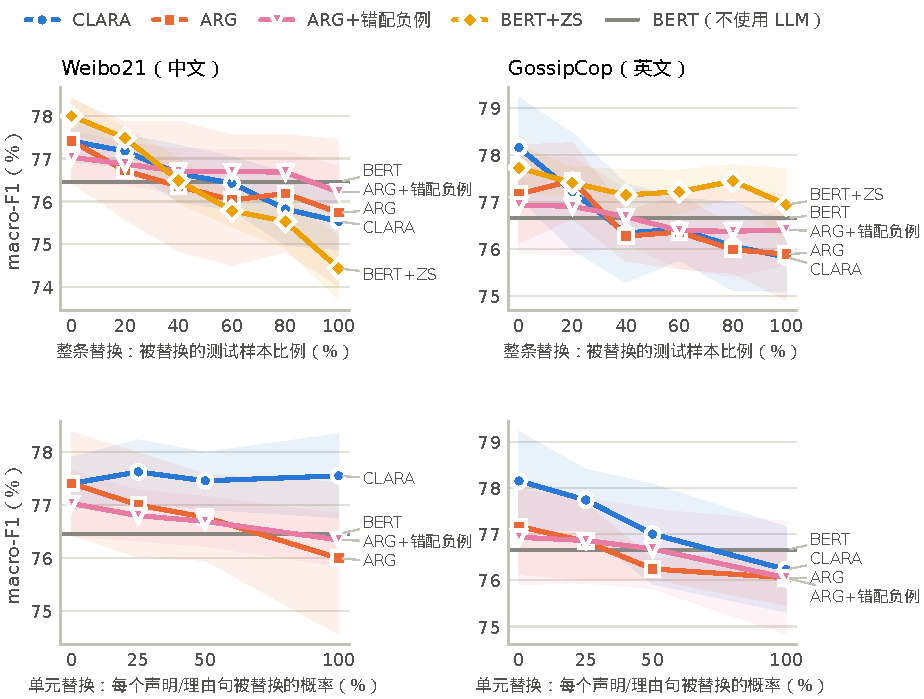
\includegraphics[width=\linewidth]{figures/noise.pdf}
\caption{LLM 分析被替换时的 macro-F1。上：整条替换；下：单元替换。阴影为种子间标准差，灰色横线为不使用 LLM 的 BERT。数值见表~\ref{tab:noise}。}\label{fig:noise}
\end{figure}

\paragraph{相关性门控能识别不属于该新闻的分析}
表~\ref{tab:gate} 显示，相关性门控 $r$ 几乎完美地区分了属于本新闻的分析单元与被替换进来的单元：整条替换时 AUC 为 \fthree{CN/gate/relevance/item/auc_r}（Weibo21）与 \fthree{EN/gate/relevance/item/auc_r}（GossipCop），单元替换时为 \fthree{CN/gate/relevance/unit/auc_r} 与 \fthree{EN/gate/relevance/unit/auc_r}。属于本新闻的单元平均 $r$ 在 0.93 以上，被替换的单元在 0.2 以下。判定门控 $g$ 则完全不具备这一能力（AUC 约 0.5）。

\begin{table}[t]
\centering\small
\caption{相关性门控对“分析单元是否属于该新闻”的区分能力（测试集，多种子均值）。}\label{tab:gate}
\begin{tabular}{lcccc}
\toprule
 & \multicolumn{2}{c}{Weibo21（中文）} & \multicolumn{2}{c}{GossipCop（英文）} \\
\cmidrule(lr){2-3}\cmidrule(lr){4-5}
 & 整条替换 & 单元替换 & 整条替换 & 单元替换 \\
\midrule
AUC：相关性门控 $r$ $\rightarrow$ 是否为本新闻的分析 & 0.996 & 0.992 & 0.994 & 0.989 \\
AUC：判定门控 $g$ $\rightarrow$ 同上 & 0.537 & 0.516 & 0.501 & 0.499 \\
本新闻的分析单元上的平均 $r$ & 0.930 & 0.958 & 0.947 & 0.957 \\
被替换的分析单元上的平均 $r$ & 0.169 & 0.098 & 0.182 & 0.132 \\
\bottomrule
\end{tabular}

\end{table}

\paragraph{去掉相关性门控后模型在替换下崩溃}
消融实验（表~\ref{tab:ablation}）中“去掉相关性门控与错配负例”的变体，在全部分析被整条替换时，Weibo21 上的 macro-F1 从 \ptwo{CN/ablation/full/noise100/mean} 降到 \ptwo{CN/ablation/no_relevance/noise100/mean}，远低于不使用 LLM 的 BERT。加入相关性门控后，\method{} 在同样条件下保持在 \ptwo{CN/noise/clara/item/100/mean}（Weibo21）与 \ptwo{EN/noise/clara/item/100/mean}（GossipCop），比 BERT 低约 1 个点。

\paragraph{单元替换是声明级结构有优势的地方}
当分析中只有一部分单元被替换时，\method{} 可以逐条丢弃无关的声明、保留其余部分。在 Weibo21 上，即使全部声明都被替换，\method{} 的 macro-F1 仍为 \ptwo{CN/noise/clara/unit/100/mean}，与未替换时（\ptwo{CN/noise/clara/unit/0/mean}）持平：此时裁决器依靠未被替换的整体判断与文本分支。ARG 在同样条件下从 \ptwo{CN/noise/arg/unit/0/mean} 降到 \ptwo{CN/noise/arg/unit/100/mean}，两者在该条件下的差异显著（配对 bootstrap，$p=\fthree{CN/noise_sig/unit100/arg/bootstrap/p}$）。GossipCop 上没有这一优势：\method{} 从 \ptwo{EN/noise/clara/unit/0/mean} 降到 \ptwo{EN/noise/clara/unit/100/mean}，降幅大于 ARG（\ptwo{EN/noise/arg/unit/0/mean} 降到 \ptwo{EN/noise/arg/unit/100/mean}），两者最终水平相当。

\paragraph{需要如实说明的两点}
第一，ARG 本身对替换就相当稳健：整条替换全部理由后，它在两个数据集上只下降 1.3--1.7 个点。它的融合权重并不能识别被替换的理由（被替换与未被替换样本上的平均权重几乎相同，区分两者的 AUC 为 \fthree{CN/gate/weights_under_noise/arg/auc} 与 \fthree{EN/gate/weights_under_noise/arg/auc}），稳健性来自新闻文本在其表示中占主导。给 ARG 加上同样的错配负例训练后，它在整条替换下略好于 \method{}。因此，“在分析不可用时保持稳健”并不是 \method{} 独有的性质；\method{} 相对 ARG 的可测优势只出现在 Weibo21 的单元替换上。第二，FactGuard 对两种替换都非常敏感（整条替换全部分析后降到 \ptwo{CN/noise/factguard/item/100/mean} 与 \ptwo{EN/noise/factguard/item/100/mean}），因为它用 LLM 抽取的 topic-content 代替新闻原文参与交叉注意力。

\subsection{判定门控学到了什么}\label{sec:exp-gate}

判定门控 $g$ 的设计意图是估计“LLM 在该实例上是否站对了边”。表~\ref{tab:gate-cells} 按 LLM 的整体判断与新闻标签把测试样本分为四组，给出各组的平均 $g_0$。

\begin{table}[t]
\centering\small
\caption{判定门控在整体实例上的取值（测试集，多种子均值）。若门控跟随“LLM 是否正确”，则第一、四行应高，第二、三行应低。}\label{tab:gate-cells}
\begin{tabular}{llcccc}
\toprule
 & & \multicolumn{2}{c}{Weibo21（中文）} & \multicolumn{2}{c}{GossipCop（英文）} \\
\cmidrule(lr){3-4}\cmidrule(lr){5-6}
LLM 的整体判断 & 新闻标签 & 占比（\%） & 平均 $g_0$ & 占比（\%） & 平均 $g_0$ \\
\midrule
判假 & 假（LLM 对） & 33.6 & 0.805 & 5.3 & 0.564 \\
判假 & 真（LLM 错） & 17.6 & 0.656 & 7.3 & 0.815 \\
判真 & 假（LLM 错） & 8.1 & 0.810 & 13.1 & 0.692 \\
判真 & 真（LLM 对） & 40.7 & 0.625 & 74.3 & 0.842 \\
\midrule
\multicolumn{2}{l}{AUC：$g_0$ $\rightarrow$ LLM 的整体判断是否正确} & \multicolumn{2}{c}{0.482} & \multicolumn{2}{c}{0.680} \\
\multicolumn{2}{l}{AUC：$g_0$ $\rightarrow$ 新闻是否为假} & \multicolumn{2}{c}{0.745} & \multicolumn{2}{c}{0.192} \\
\multicolumn{2}{l}{AUC：LLM 自身置信度 $\rightarrow$ 判断是否正确} & \multicolumn{2}{c}{0.532} & \multicolumn{2}{c}{0.510} \\
\multicolumn{2}{l}{AUC：文本分支与 LLM 是否一致 $\rightarrow$ 判断是否正确} & \multicolumn{2}{c}{0.760} & \multicolumn{2}{c}{0.858} \\
\bottomrule
\end{tabular}

\end{table}

\paragraph{判定门控跟随的是新闻标签，而不是 LLM 的正误}
在 Weibo21 上，$g_0$ 在两组假新闻上都高（约 0.81），在两组真新闻上都低（约 0.63--0.66），与 LLM 判断的方向无关：它预测“LLM 是否正确”的 AUC 为 \fthree{CN/gate/clara/overall/auc_gate/mean}，预测“新闻是否为假”的 AUC 却有 \fthree{CN/gate/clara/overall/auc_gate_for_label/mean}。在 GossipCop 上情形相反，$g_0$ 在真新闻上更高，对“LLM 是否正确”的 AUC 为 \fthree{EN/gate/clara/overall/auc_gate/mean}，但这同样可以由标签解释：该数据集上 LLM 多数时候判真，“LLM 正确”与“新闻为真”高度重合。也就是说，一个能看到新闻文本的门控学到的是“这条新闻像不像假新闻”，并据此调节 LLM 证据的权重。它起到的是让 LLM 证据的权重随文本先验变化的作用，而不是可靠性估计。

\paragraph{这一现象并非 \method{} 独有}
ARG 的理由可用性预测器对“该理由对应的 LLM 判断是否正确”的 AUC 看起来不低（表~\ref{tab:useful}），但决定融合权重的打分模块对同一目标的 AUC 只有 0.50--0.55。可用性预测器同时读取新闻与理由：新闻文本提示标签，理由文本提示 LLM 的判断，两者一比较即可得到监督目标。表中“自身预测”一列用 ARG 最终的预测概率与 LLM 判断是否一致来预测同一目标，不需要任何专门的模块，得到的 AUC 与可用性预测器相当或更高。可见可用性预测器并没有提供分类器自身判断之外的信息。

\begin{table}[t]
\centering\small
\caption{对“该理由对应的 LLM 判断是否正确”的 AUC（测试集，多种子均值）：ARG 的可用性预测器、融合权重，以及“ARG 自身的最终预测与 LLM 判断是否一致”。}\label{tab:useful}
\begin{tabular}{llcccccc}
\toprule
 & & \multicolumn{3}{c}{Weibo21（中文）} & \multicolumn{3}{c}{GossipCop（英文）} \\
\cmidrule(lr){3-5}\cmidrule(lr){6-8}
模型 & 理由 & 可用性预测 & 融合权重 & 自身预测 & 可用性预测 & 融合权重 & 自身预测 \\
\midrule
ARG & 文字描述 & 0.757 & 0.548 & 0.778 & 0.882 & 0.521 & 0.887 \\
 & 常识 & 0.762 & 0.500 & 0.796 & 0.913 & 0.523 & 0.910 \\
ARG + 错配负例 & 文字描述 & 0.754 & 0.452 & 0.774 & 0.877 & 0.666 & 0.885 \\
 & 常识 & 0.773 & 0.550 & 0.790 & 0.902 & 0.575 & 0.908 \\
\bottomrule
\end{tabular}

\end{table}

\paragraph{LLM 自身的置信度也不提供这一信息}
LLM 评分偏离 0.5 的程度对其判断是否正确的 AUC 只有 \fthree{CN/gate/clara/overall/auc_llm_conf/mean} 与 \fthree{EN/gate/clara/overall/auc_llm_conf/mean}。真正有信息量的是“文本分支是否同意 LLM”（AUC \fthree{CN/gate/clara/overall/auc_text_agreement/mean} 与 \fthree{EN/gate/clara/overall/auc_text_agreement/mean}），而这一信息在加性融合中已经被隐式使用。综合来看，在闭卷条件下我们没有找到能够估计“LLM 的判断是否可靠”且不退化为预测标签的信号；本文最初设想的“声明级可靠性门控”在这一含义上没有成立，成立的是相关性门控所回答的那个更窄的问题。

\paragraph{实例概率的分布}
两个数据集上承担判定的实例不同。在 Weibo21 的假新闻中，至少有一条声明 $p_k>0.5$ 的占 \pone{CN/gate/clara/flag/fake_any_claim/mean}\%，只有整体实例 $p_0>0.5$ 的占 \pone{CN/gate/clara/flag/fake_overall_only/mean}\%，可见这里新闻级的判定主要由整体实例承担。在 GossipCop 的假新闻中，至少有一条声明 $p_k>0.5$ 的占 \pone{EN/gate/clara/flag/fake_any_claim/mean}\%，而只由整体实例触发的不到 1\%：该数据集上 LLM 的整体判断区分度很低（零样本判断的 AUC 仅 \pone{EN/style_llm/zero-shot P(fake)/auc_orig}\%），裁决器转而依靠声明实例。

\subsection{风格改写}\label{sec:exp-style}

\begin{table}[t]
\centering\small
\caption{风格改写前后的 macro-F1（\%）。只统计成功改写的样本，“原文”为同一批样本改写前的结果。分隔线以下两行是只读取 LLM 输出文本、不读新闻原文的 BERT。}\label{tab:style}
\begin{tabular}{lcccccc}
\toprule
 & \multicolumn{3}{c}{Weibo21（中文）} & \multicolumn{3}{c}{GossipCop（英文）} \\
\cmidrule(lr){2-4}\cmidrule(lr){5-7}
方法 & 原文 & 改写后 & $\Delta$ & 原文 & 改写后 & $\Delta$ \\
\midrule
BERT & 76.09\pmstd{0.38} & 50.82\pmstd{2.03} & -25.27 & 76.66\pmstd{1.34} & 64.76\pmstd{1.72} & -11.89 \\
LoRA-LLM & 79.90\pmstd{1.09} & \textbf{60.56}\pmstd{1.07} & -19.34 & 77.04\pmstd{0.56} & \textbf{72.64}\pmstd{0.65} & -4.40 \\
BERT+ZS & 77.70\pmstd{0.56} & 52.62\pmstd{1.43} & -25.08 & 77.73\pmstd{0.47} & 66.80\pmstd{1.71} & -10.92 \\
ARG & 77.10\pmstd{0.90} & 50.94\pmstd{5.14} & -26.16 & 77.17\pmstd{1.04} & 64.91\pmstd{1.26} & -12.26 \\
FactGuard & 75.90\pmstd{0.82} & 53.26\pmstd{4.18} & -22.64 & 77.24\pmstd{1.01} & 68.79\pmstd{1.97} & -8.45 \\
\method{} & 77.35\pmstd{0.46} & 53.08\pmstd{2.13} & -24.28 & 78.15\pmstd{1.06} & 68.06\pmstd{0.45} & -10.09 \\
\student{} & 75.53\pmstd{0.79} & 50.15\pmstd{1.15} & -25.37 & -- & -- & -- \\
\bottomrule
\end{tabular}

\end{table}

\paragraph{所有闭卷检测器都主要依赖文风}
把假新闻改写为通稿文风、真新闻改写为营销号文风后，Weibo21 上所有 SLM 类方法的 macro-F1 从 76--78 降到 51--53，接近随机；GossipCop 上从约 77 降到 65--69（表~\ref{tab:style}）。在 Weibo21 上各 SLM 类方法改写后的差异都在种子波动之内；在 GossipCop 上，FactGuard 与 \method{} 改写后比 BERT 高约 3--4 个点，这两种方法都使用了 LLM 对新闻内容的重新表述（topic-content 或声明），其文风与原文不同。直接微调的 LoRA-LLM 下降较少，但同样明显。

\paragraph{LLM 自身的判断同样依赖文风}
表~\ref{tab:style-llm} 不涉及任何训练，只比较 Qwen2.5-7B 对同一批样本改写前后的评分。零样本判断的 AUC 在 Weibo21 上从 \pone{CN/style_llm/zero-shot P(fake)/auc_orig} 降到 \pone{CN/style_llm/zero-shot P(fake)/auc_style}，在 GossipCop 上从 \pone{EN/style_llm/zero-shot P(fake)/auc_orig} 降到 \pone{EN/style_llm/zero-shot P(fake)/auc_style}。声明级怀疑度在改写后对真假新闻几乎没有区分度。这说明 LLM 在闭卷条件下给出的“常识分析”“声明核查”，其判别力主要来自文本的表面特征，而不是对事实的掌握。把 LLM 的分析拆得更细并不能改变这一点：声明是从改写后的文本中抽取的，其措辞与评分仍然随文风变化。

\begin{table}[t]
\centering\small
\caption{Qwen2.5-7B 的评分在风格改写前后对真假新闻的区分能力（不涉及训练）。均值差为假新闻与真新闻平均评分之差。}\label{tab:style-llm}
\begin{tabular}{lcccccccc}
\toprule
 & \multicolumn{4}{c}{Weibo21（中文）} & \multicolumn{4}{c}{GossipCop（英文）} \\
\cmidrule(lr){2-5}\cmidrule(lr){6-9}
 & \multicolumn{2}{c}{AUC（\%）} & \multicolumn{2}{c}{均值差（假$-$真）} & \multicolumn{2}{c}{AUC（\%）} & \multicolumn{2}{c}{均值差（假$-$真）} \\
LLM 评分 & 原文 & 改写 & 原文 & 改写 & 原文 & 改写 & 原文 & 改写 \\
\midrule
零样本判断 $p_{\mathrm{zs}}$ & 83.2 & 58.7 & 0.50 & 0.13 & 67.4 & 50.9 & 0.20 & 0.04 \\
整体判断的怀疑度 $v_0$ & 75.8 & 54.9 & 0.13 & 0.02 & 65.6 & 57.0 & 0.06 & 0.03 \\
声明怀疑度的最大值 & 71.0 & 50.7 & 0.11 & 0.00 & 58.5 & 56.0 & 0.03 & 0.02 \\
声明怀疑度的均值 & 72.6 & 51.2 & 0.11 & 0.01 & 56.2 & 52.7 & 0.02 & 0.01 \\
\bottomrule
\end{tabular}

\end{table}

\subsection{单句事实篡改：敏感性与定位}\label{sec:exp-loc}

\begin{table}[t]
\centering\small
\caption{对单句事实篡改的敏感性（\%）。“判假”为被判为假的比例；成对正确率为篡改后样本的预测概率高于其原文的比例，50\% 相当于随机。}\label{tab:tamper}
\begin{tabular}{lcccccc}
\toprule
 & \multicolumn{3}{c}{Weibo21（中文）} & \multicolumn{3}{c}{GossipCop（英文）} \\
\cmidrule(lr){2-4}\cmidrule(lr){5-7}
方法 & 原文判假 & 篡改后判假 & 成对正确率 & 原文判假 & 篡改后判假 & 成对正确率 \\
\midrule
BERT & 22.7 & 22.9 & 54.6 & 9.0 & 9.2 & 53.4 \\
LoRA-LLM & 15.7 & 18.2 & 68.8 & -- & -- & -- \\
BERT+ZS & 21.8 & 23.4 & 60.6 & 6.1 & 6.4 & 57.4 \\
ARG & 19.3 & 19.7 & 55.4 & 7.5 & 7.9 & 53.5 \\
FactGuard & 22.0 & 23.1 & 54.1 & 8.3 & 8.8 & 53.3 \\
\method{} & 20.0 & 21.1 & 54.8 & 8.0 & 8.6 & 53.1 \\
\bottomrule
\end{tabular}

\end{table}

\paragraph{没有方法对局部事实改动敏感}
表~\ref{tab:tamper} 显示，把真新闻中的一句话改成与原文事实不符的陈述后，各方法判其为假的比例几乎不变（例如 \method{} 在 Weibo21 上从 \pone{CN/localisation/_sensitivity/clara/flag_rate_original}\% 变为 \pone{CN/localisation/_sensitivity/clara/flag_rate_tampered}\%）；篡改后的预测概率高于原文的比例只有 53\%--55\%，略高于随机。唯一稍高的是 BERT+ZS（约 57\%--61\%），因为 LLM 的零样本评分对部分改动有反应。这与风格改写的结果一致：这些检测器学到的不是“内容是否属实”。需要强调，篡改后的句子只是与原文不符，未必在现实中为假，这项测试衡量的是模型对事实内容变化的敏感程度。

\begin{table}[t]
\centering\small
\caption{被篡改句子的定位结果（\%）。“单位”为方法给出分数的粒度；声明级分数通过声明所在的句子编号映射到句子。}\label{tab:loc}
\begin{tabular}{llcccc}
\toprule
 & & \multicolumn{2}{c}{Weibo21（中文）} & \multicolumn{2}{c}{GossipCop（英文）} \\
\cmidrule(lr){3-4}\cmidrule(lr){5-6}
方法 & 单位 & Hit@1 & MRR & Hit@1 & MRR \\
\midrule
随机猜测 & 句子 & 30.0 & -- & 19.8 & -- \\
LLM 怀疑度评分（不训练） & 声明 & 35.7 & 59.2 & 22.8 & 47.1 \\
BERT + 遮挡归因 & 句子 & 33.2\pmstd{1.2} & 58.4 & 22.2\pmstd{1.0} & 46.5 \\
LoRA-LLM + 遮挡归因 & 句子 & 38.3\pmstd{1.0} & 61.9 & 24.0\pmstd{1.9} & 48.4 \\
\method{} & 声明 & 36.2\pmstd{0.8} & 59.6 & 23.2\pmstd{0.6} & 47.0 \\
\midrule
\method{}：去掉论证文本 & 声明 & 35.4\pmstd{0.7} & 59.2 & -- & -- \\
\method{}：去掉评分 & 声明 & 35.1\pmstd{0.8} & 59.0 & -- & -- \\
\bottomrule
\end{tabular}

\end{table}

\paragraph{定位结果只略高于随机}
在定位任务上（表~\ref{tab:loc}），\method{} 的 Hit@1 在 Weibo21 上为 \pone{CN/localisation/CLARA/hit@1}\%，随机猜测为 \pone{CN/localisation/CLARA/chance}\%；在 GossipCop 上为 \pone{EN/localisation/CLARA/hit@1}\%，随机为 \pone{EN/localisation/CLARA/chance}\%。训练后的裁决器并没有比直接使用 LLM 的怀疑度评分更好，与对 BERT 做遮挡归因也相差无几。原因有两个：LLM 抽取的声明只覆盖了 \pone{CN/localisation/_claim_coverage}\%（Weibo21）与 \pone{EN/localisation/_claim_coverage}\%（GossipCop）的被篡改句子；即使覆盖到，LLM 对这条声明的怀疑度也往往不比其他声明高。“只用新闻级标签即可获得声明级定位”这一预期在闭卷条件下没有实现。

\subsection{消融实验}\label{sec:exp-ablation}

\begin{table}[t]
\centering\footnotesize
\setlength{\tabcolsep}{3.4pt}
\caption{\method{} 的消融（macro-F1，\%）。“整条替换”为全部测试样本的分析被替换，“半数单元替换”为每个单元以 0.5 的概率被替换。Weibo21 为 5 个种子，GossipCop 为 3 个种子。$^{*}$ 表示与完整模型的差异在配对 bootstrap 检验下显著（$p<0.05$）。}\label{tab:ablation}
\begin{tabular}{lcccccc}
\toprule
\multirow{2}{*}{变体} & \multicolumn{3}{c}{Weibo21（中文）} & \multicolumn{3}{c}{GossipCop（英文）} \\
\cmidrule(lr){2-4}\cmidrule(lr){5-7}
 & 原始 & 整条替换 & 单元替换 & 原始 & 整条替换 & 单元替换 \\
\midrule
\method{}（完整） & 77.41\pmstd{0.49} & 75.53\pmstd{0.66} & 77.55\pmstd{0.79} & -- & -- & -- \\
\midrule
去掉声明，仅整体实例 & 77.24\pmstd{0.53} & 74.90\pmstd{0.70} & 77.24\pmstd{0.53} & -- & -- & -- \\
去掉整体实例，仅声明 & 76.91\pmstd{0.39} & 75.48\pmstd{0.43} & 75.40\pmstd{0.31}$^{*}$ & -- & -- & -- \\
\midrule
去掉论证文本，仅评分 & 77.19\pmstd{0.36} & 75.14\pmstd{0.36} & 77.31\pmstd{0.32} & -- & -- & -- \\
去掉评分，仅论证文本 & 75.79\pmstd{0.71}$^{*}$ & 75.93\pmstd{0.61} & 75.63\pmstd{0.66}$^{*}$ & -- & -- & -- \\
论证前评分取提示内第一印象（严格单次调用） & 76.29\pmstd{0.43} & 75.26\pmstd{0.24} & 76.33\pmstd{0.52} & -- & -- & -- \\
\bottomrule
\end{tabular}

\end{table}

表~\ref{tab:ablation} 给出各组件的消融结果，详见 \ref{sec:exp-ablation-text} 节。

\subsection{未见领域}\label{sec:exp-lodo}

\begin{table}[t]
\centering\small
\caption{Weibo21 留一领域实验的 macro-F1（\%，3 个种子）。训练与验证数据不含被留出的领域。}\label{tab:lodo}
\begin{tabular}{lrrcccc}
\toprule
留出领域 & 训练数 & 测试数 & BERT & BERT+ZS & ARG & \method{} \\
\midrule
医药健康 & 4,100 & 271 & 73.82\pmstd{0.76} & \textbf{79.96}\pmstd{0.97} & 76.69\pmstd{2.41} & 75.02\pmstd{3.06} \\
政治 & 3,950 & 126 & 76.42\pmstd{3.30} & \textbf{79.59}\pmstd{0.44} & 77.75\pmstd{0.80} & 76.69\pmstd{1.22} \\
文体娱乐 & 3,444 & 134 & \textbf{73.38}\pmstd{2.86} & 71.43\pmstd{0.92} & 68.66\pmstd{2.44} & 70.64\pmstd{0.68} \\
灾难事故 & 4,135 & 185 & \textbf{79.05}\pmstd{1.60} & 78.84\pmstd{1.66} & 78.70\pmstd{1.27} & 77.78\pmstd{1.59} \\
社会生活 & 2,952 & 391 & 75.99\pmstd{1.05} & \textbf{78.74}\pmstd{0.67} & 78.04\pmstd{0.85} & 76.17\pmstd{0.46} \\
财经商业 & 3,997 & 344 & 53.62\pmstd{3.04} & \textbf{56.52}\pmstd{3.41} & 54.14\pmstd{0.53} & 56.48\pmstd{0.77} \\
\midrule
各领域平均 & & & 72.05 & \textbf{74.18}$^{*}$ & 72.33 & 72.13 \\
\bottomrule
\end{tabular}

\end{table}

\subsection{拒答}\label{sec:exp-selective}

\begin{table}[t]
\centering\small
\caption{选择性预测。AURC 越低越好；Acc@$c$ 为保留置信度最高的 $c\%$ 样本时的准确率（\%）。“选择器”为在验证集上拟合的逻辑回归。}\label{tab:selective}
\begin{tabular}{lcccccc}
\toprule
 & \multicolumn{3}{c}{Weibo21（中文）} & \multicolumn{3}{c}{GossipCop（英文）} \\
\cmidrule(lr){2-4}\cmidrule(lr){5-7}
方法 & AURC$\downarrow$ & Acc@90 & Acc@70 & AURC$\downarrow$ & Acc@90 & Acc@70 \\
\midrule
BERT & 13.75 & 79.23 & 83.25 & 6.26 & 88.60 & 91.99 \\
LoRA-LLM & 7.37 & 82.63 & 89.68 & -- & -- & -- \\
BERT+ZS & 14.44 & 80.64 & 84.14 & 5.08 & 89.88 & 92.92 \\
ARG & 12.69 & 80.40 & 85.01 & 6.77 & 89.29 & 92.83 \\
ARG + 选择器 & 12.28 & 79.87 & 83.25 & 5.97 & 89.47 & 93.35 \\
FactGuard & 17.52 & 78.93 & 82.66 & 6.50 & 89.19 & 92.26 \\
FactGuard + 选择器 & 14.57 & 78.58 & 80.85 & 6.06 & 89.29 & 92.53 \\
\method{} & 15.86 & 80.28 & 84.17 & 6.52 & 89.58 & 92.62 \\
\method{} + 选择器 & 11.11 & 80.13 & 83.51 & 5.81 & 89.68 & 93.64 \\
\bottomrule
\end{tabular}

\end{table}

\begin{figure}[t]
\centering
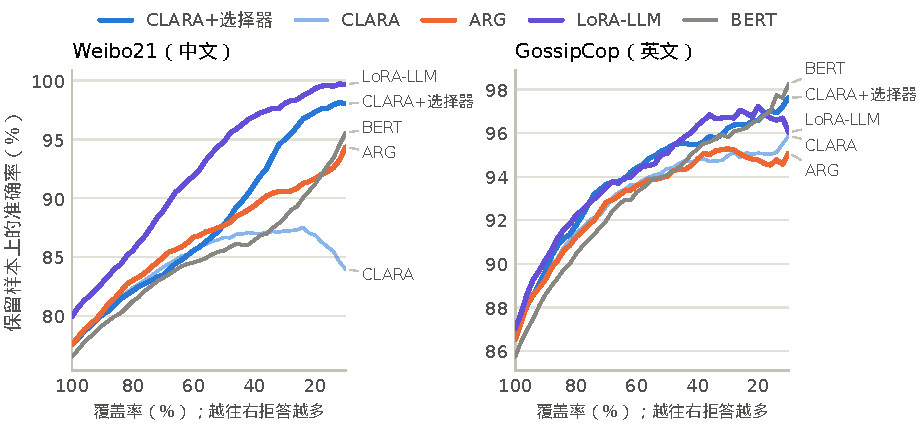
\includegraphics[width=\linewidth]{figures/selective.pdf}
\caption{保留样本上的准确率随覆盖率的变化（多种子均值）。数值见表~\ref{tab:selective}。}\label{fig:selective}
\end{figure}

\subsection{开销}\label{sec:exp-cost}

\begin{table}[t]
\centering\small
\caption{每条新闻的 LLM 开销：平均输入与输出 token 数，以及单张 RTX 3090 上用 vLLM 批量生成时每千条新闻的耗时。}\label{tab:cost}
\begin{tabular}{lccccccc}
\toprule
 & & \multicolumn{3}{c}{Weibo21（中文）} & \multicolumn{3}{c}{GossipCop（英文）} \\
\cmidrule(lr){3-5}\cmidrule(lr){6-8}
LLM 输出 & 调用数 & 输入 & 输出 & 秒/千条 & 输入 & 输出 & 秒/千条 \\
\midrule
零样本判断 & 1 & 133 & 2 & 17 & 224 & 2 & 34 \\
ARG（TD + CS 理由） & 2 & 317 & 208 & 125 & 511 & 140 & 140 \\
FactGuard（topic-content + CS 理由） & 2 & 487 & 158 & 104 & 820 & 163 & 152 \\
\method{}（结构化调用 + 零样本评分） & 2 & 791 & 283 & 182 & 984 & 438 & 319 \\
\method{}，严格单次调用 & 1 & 657 & 281 & 166 & 759 & 436 & 284 \\
\bottomrule
\end{tabular}

\end{table}

\begin{table}[t]
\centering\small
\caption{可训练参数量与单次训练耗时（单张 RTX 3090；SLM 类方法不含冻结层的一次性缓存）。}\label{tab:train-cost}
\begin{tabular}{lrrr}
\toprule
方法 & 可训练参数（M） & 训练秒数（CN） & 训练秒数（EN） \\
\midrule
BERT & 7.4 & 15 & 8 \\
BERT+ZS & 7.4 & 14 & 9 \\
ARG & 25.8 & 110 & 52 \\
FactGuard & 25.7 & 130 & 57 \\
\method{} & 20.7 & 136 & 106 \\
LoRA-LLM & 40.4 & 1940 & -- \\
\bottomrule
\end{tabular}

\end{table}

\section{讨论}\label{sec:discussion}

\paragraph{为什么判定门控学不到“LLM 是否可靠”}
“LLM 在某个实例上是否站对了边”由两个量决定：LLM 表达的判断与该实例的真实状态。前者写在 LLM 的输出里，后者在闭卷条件下只能由新闻文本去推测。因此，一个读取新闻文本与 LLM 输出的门控，要预测这一目标，最直接的办法就是先从文本预测标签，再与 LLM 的判断比较。表~\ref{tab:gate-cells} 与表~\ref{tab:useful} 显示 \method{} 的判定门控与 ARG 的可用性预测器都落在这一解上。要得到不依赖标签预测的可靠性估计，需要第三个信息来源，例如外部证据，或 LLM 在同一问题上多次采样的一致性；后者是否有效留待后续工作检验。多示例学习的不对称性确实为真新闻中的声明提供了精确的监督，但这一监督同样可以由“这是一条真新闻”推出，并没有迫使模型去判断单条声明。

\paragraph{多示例假设在多大程度上成立}
式~\eqref{eq:mil} 假设假新闻中存在可以单独指认的问题声明。\ref{sec:exp-gate} 节的统计显示，在 Weibo21 上多数假新闻是由整体实例而不是某条声明触发的。这与数据的性质有关：社交媒体上的不实消息常常整体是编造的，其中每条声明单独看都“像是可能发生的”，仅凭文本无法指出哪一条有问题。反过来，真新闻如实转述不实说法的情形会违反假设的另一半；我们在提示词中要求保留归属以减少这种情况，但没有通过人工标注去度量假设被违反的比例，这是本文的一个局限。

\paragraph{关于任务本身}
风格改写与事实篡改两项测试指向同一个结论：在这两个常用数据集上，闭卷检测器学到的主要是真假新闻在写法上的差异。这与 \citet{wu2024sheepdog} 对 SLM 的观察一致，本文进一步表明它同样适用于 LLM 的闭卷判断，以及建立在这些判断之上的协同方法。把 LLM 的分析拆得更细、让它写出正反论证，改变的是分析的形式，而没有改变分析所依据的信息。对于“内容是否属实”这一问题，闭卷的 7B 模型既不掌握所需的事实，也没有表现出能从文本内部一致性中发现问题的能力。这提示：在不引入外部证据的前提下继续改进 LLM 与 SLM 的协同结构，在这类基准上能得到的主要是对文风线索更充分的利用；而声称具备“事实分析”能力的闭卷方法，应当接受风格受控的测试。

\paragraph{对实践的建议}
如果目标只是分布内精度：在算力允许时直接微调 LLM；否则在 SLM 的输出上融合一个 LLM 零样本评分，成本最低且不逊于更复杂的结构。如果系统中确实要使用 LLM 生成的分析文本，本文的结果支持为它配一个相关性检查：它几乎不损失精度，却能避免在分析与新闻不符时性能大幅下降。无论采用哪种方案，方法间 1 个点以内的差异都需要多个随机种子与显著性检验才能判断。

\paragraph{局限}
（1）分析用的 LLM 以 Qwen2.5-7B 为主，更强的模型可能掌握更多事实，结论未必外推到闭源大模型。（2）只使用了两个数据集，且都来自同一来源的时间划分。（3）风格改写与事实篡改由另一个 LLM 自动生成，事实是否保持只用数字串的保留比例做了粗略检查，没有人工核验；篡改后的句子与原文不符，但未必在现实中为假。（4）\method{} 的第一个版本曾在测试集上评估过一次，相关性门控是在看到那次结果后加入的（\ref{sec:protocol} 节）；虽然此后的选择只依据验证集，这仍然弱化了测试集的独立性。（5）本文对 ARG 的复现比其官方代码低 0.5--1 个点。（6）声明的质量、论证的质量以及定位结果都没有做人工评估。（7）\method{} 的超参数没有搜索，可能不是最优。

\section{结论}\label{sec:conclusion}

本文研究闭卷条件下如何利用 LLM 的分析来检测虚假新闻。我们提出 \method{}：LLM 把新闻分解为声明并为每条声明写出正反两方论证，可训练的裁决器以声明为实例做多示例学习，用相关性门控剔除不属于该新闻的分析单元，并在所有单元都不可用时退回到只依赖文本的判断。我们在统一了 LLM、超参数搜索与随机种子的条件下，把它与 ARG、FactGuard、直接微调的 LLM 以及一个简单的评分融合基线做了比较，并设计了四项受控测试。

结论有三层。第一，就方法而言，\method{} 在分布内与已有的协同方法持平；它的相关性门控是有效的，能可靠地识别与新闻对不上的分析单元，但这回答的只是“分析是否属于这条新闻”，而不是“分析是否正确”。第二，就这一类方法而言，我们没有找到能在闭卷条件下估计“LLM 的判断是否可靠”的信号：\method{} 的判定门控与 ARG 的可用性机制实际学到的都是对新闻标签的预测。第三，就任务而言，风格改写与事实篡改两项测试表明，包括 LLM 自身判断在内的所有闭卷检测器主要依赖文风，对内容层面的事实改动几乎没有反应；把 LLM 的分析做得更细、更结构化，并不能改变它所依据的信息。

这些结果指向两个后续方向。其一，要让检测器真正对“内容是否属实”作出反应，需要引入模型参数之外的信息，例如检索到的证据；本文的声明分解与相关性门控可以直接用于判断检索到的证据是否与某条声明相关。其二，评测上，闭卷检测方法应当在风格受控与事实受控的测试集上报告结果，并与“直接微调同一个 LLM”以及“融合一个 LLM 评分”这两个基线比较；在多随机种子的设置下，1 个点以内的差距不足以支撑结论。


\bibliographystyle{unsrtnat}
\bibliography{refs}

\appendix
\section{提示词}\label{app:prompt}

\paragraph{声明分解与双立场论证（中文）}
下面是 \method{} 结构化调用的系统提示与用户提示。$a^+$ 与 $a^-$ 的书写顺序按样本编号的奇偶交替，这里给出先写支持论证的版本。输出受 JSON schema 约束，字段依次为 \texttt{first\_impression}、\texttt{claims}（每条含 \texttt{claim}、\texttt{type}、\texttt{sent}、两条论证与 \texttt{suspicion}）和 \texttt{overall}。

{\small\setlength{\parindent}{0pt}\begin{quote}
你是一名严谨的事实核查分析员。你无法联网检索，只能依据消息文本本身以及你已有的常识和背景知识进行分析。\par
\vspace{3pt}
下面是一条已按句编号的新闻或社交媒体消息。请对它做“声明分解 + 正反论证”分析，只输出一个 JSON 对象。\par
\vspace{3pt}
【步骤】\par
0. 先不做分析，凭第一印象填写 first\_impression：整条消息是虚假或误导性信息的可能性，1=几乎肯定属实，2=较可能属实，3=无法判断，4=较可能不实，5=几乎肯定不实。\par
1. 找出消息中最核心、可被核查的原子声明（claim），按重要性排序，共 1–6 条，尽量覆盖消息中彼此不同的事实陈述。\par
\hspace*{3em}- 一条声明只陈述一件事，并且要自包含：补全主语、时间、地点，不要出现“他”“该公司”“此事”等指代。\par
\hspace*{3em}- 保留归属：原文若是“某人/某机构称……”，声明里必须保留“某人称”，不要改写成既成事实。\par
\hspace*{3em}- 不要抽取情绪宣泄、呼吁转发、提问、投票等非事实内容。\par
2. 对每条声明写出两条有针对性的理由，各不超过 60 字：\par
\hspace*{3em}- support：认为这条声明可信的最强理由；\par
\hspace*{3em}- refute：认为这条声明可疑的最强理由。\par
\hspace*{3em}理由要结合常识、背景知识、逻辑和文本内部的一致性，针对这条声明本身来写，避免“细节具体”“缺乏来源”这类对任何消息都适用的套话；不要写“所以这是真/假新闻”之类的结论。\par
3. 写完两条理由后，权衡哪一方更站得住脚，再给出 suspicion（该声明不属实的可能性）：\par
\hspace*{3em}1–5，含义同第 0 步。\par
4. type：fact=事件或事实陈述，number=数字或统计，quote=引述他人说法，opinion=预测、评价或观点。\par
5. sent：这条声明主要出自哪一句（填句子编号）。\par
6. 最后填写 overall（整体判断）：综合上面各条声明的分析，并考虑标题与正文是否一致、信息来源是否明确可靠、是否煽动情绪或夸大其词、叙述是否自洽，对整条消息做出评估。同样先写 support（认为整条消息可信的最强理由）和 refute（认为整条消息不可信的最强理由），再给出 suspicion（整条消息是虚假或误导性信息的可能性，1–5，含义同上）。\par
\vspace{3pt}
【消息】\par
〈按句编号的消息文本：[1] …… [2] ……〉\par
\end{quote}}


\paragraph{声明分解与双立场论证（英文）}

{\small\setlength{\parindent}{0pt}\begin{quote}
You are a rigorous fact-checking analyst. You cannot search the web; rely only on the message itself and on your own commonsense and background knowledge.\par
\vspace{3pt}
Below is a news article or social media message whose sentences have been numbered. Perform a "claim decomposition + two-sided argumentation" analysis and output a single JSON object only.\par
\vspace{3pt}
Steps:\par
0. Before any analysis, fill in first\_impression from your first impression: how likely the whole message is false or misleading, 1 = almost certainly true, 2 = more likely true, 3 = cannot tell, 4 = more likely untrue, 5 = almost certainly untrue.\par
1. Extract the most central, checkable atomic claims of the message, ordered by importance: between 1 and 6 claims, covering the distinct factual assertions of the message.\par
\hspace*{3em}- Each claim states exactly one thing and must be self-contained: fill in the subject, time and place; do not use pronouns or references such as "he", "the company", "this".\par
\hspace*{3em}- Keep the attribution: if the text says "X said/claimed ...", the claim must keep "X said"; do not rewrite it as an established fact.\par
\hspace*{3em}- Do not extract emotional venting, calls to share, questions, or other non-factual content.\par
2. For each claim write two targeted arguments, each at most 40 words:\par
\hspace*{3em}- support: the strongest argument that this claim is credible;\par
\hspace*{3em}- refute: the strongest argument that this claim is doubtful.\par
\hspace*{3em}Ground the arguments in commonsense, background knowledge, logic and the internal consistency of the text, and make them specific to this claim; avoid boilerplate that would fit any message (e.g. "it gives specific details", "no source is given"). Do not state a verdict such as "so this news is real/fake".\par
3. Only after writing both arguments, weigh which side is stronger and give suspicion (how likely the claim is NOT true):\par
\hspace*{3em}1-5, same scale as in step 0.\par
4. type: fact = an event or factual statement, number = a figure or statistic, quote = a reported statement of someone, opinion = a prediction, evaluation or opinion.\par
5. sent: the number of the sentence this claim mainly comes from.\par
6. Finally fill in overall (overall judgement): combine your analysis of the claims above with whether headline and body agree, whether sources are explicit and reliable, whether the message is sensational or exaggerated, and whether the narrative is self-consistent, and assess the message as a whole. Again write support (the strongest argument that the message is credible) and refute (the strongest argument that the message is not credible) first, then give suspicion (how likely the whole message is false or misleading, 1-5, same scale as above).\par
\vspace{3pt}
Message:\par
\textless{}the message with numbered sentences: [1] ... [2] ...\textgreater{}\par
\end{quote}}


\paragraph{基线的提示词}
零样本、零样本 CoT 以及 ARG 的两个视角（文字描述、常识）使用 ARG 论文附录中的提示\citep{hu2024bad}；FactGuard 的 topic-content 抽取使用其官方仓库中的提示\citep{he2026factguard}。为便于从输出中解析判断，我们在 ARG 的提示后追加了一句长度与输出格式的要求。

\paragraph{风格改写（中文）}

{\small\setlength{\parindent}{0pt}\begin{quote}
你是一名资深编辑。\par
\vspace{3pt}
请把下面这条消息改写成〈目标文风：官方媒体通稿（如新华社、人民日报官方微博）那种客观、严谨、克制的；或：自媒体营销号、标题党那种夸张、煽情、口语化的〉文风。\par
要求：\par
1. 保留原文的全部事实信息（人物、机构、时间、地点、数字、事件、引述内容），不得增加、删除或修改任何事实；\par
2. 只改变措辞、语气和表达方式；\par
3. 篇幅与原文相近；\par
4. 只输出改写后的文本，不要任何解释。\par
\vspace{3pt}
原文：\par
〈原文〉\par
\end{quote}}


\paragraph{单句事实篡改（中文）}

{\small\setlength{\parindent}{0pt}\begin{quote}
你是一名事实核查研究助手，正在为虚假信息检测模型构造受控的测试样本。\par
\vspace{3pt}
下面给出一条消息以及其中的一句话。请对这句话做一处最小的事实性改动，使它陈述的事实与原文不同。\par
做法：从这句话里选一个尽量短的连续片段 original\_span（必须与句中文字完全一致），给出替换它的文字 new\_span；除这个片段外，句子的其余部分保持不变。\par
change\_type 说明改动类型：negation=肯定与否定互换，number=修改数字或数量，time=修改时间或日期，entity=替换人物、机构、地点或事物，outcome=颠倒结果、因果或程度。\par
要求：\par
1. 替换后的句子通顺自然；\par
2. 改动必须改变句子陈述的事实，不能是同义改写、补全残缺文字或修正错别字；\par
3. 不要加入“据说”“可能”之类的模糊词，不要改动标点。\par
只输出一个 JSON 对象。\par
\vspace{3pt}
消息全文：\par
〈消息全文〉\par
\vspace{3pt}
需要改动的句子：\par
〈被选中的句子〉\par
\end{quote}}


\section{实现细节}\label{app:impl}

\paragraph{离线生成}
LLM 输出用 vLLM\citep{kwon2023vllm} 批量生成。分析类提示（声明分解、零样本、CoT、ARG 的两个视角）采用贪心解码；topic-content 抽取沿用 FactGuard 仓库的温度 0.2；风格改写与事实篡改由 Qwen3-8B 在关闭思考模式、温度 0.3 下生成。声明分解的最大输出长度为 1{,}200 个 token，输出无法解析时以更宽松的约束重试一次。两个数据集共 15{,}522 条新闻，首次生成即可解析的比例为 \ptwo{CN/cost/clara_first_attempt_rate}\%（中文）与 \ptwo{EN/cost/clara_first_attempt_rate}\%（英文），其余在重试后全部解析成功。

\paragraph{裁决器}
隐藏层维度 384，dropout 0.2；新闻、声明、声明--论证对的最大长度分别为 170、48 与 128 个 token。优化器为 Adam（FactGuard 按其官方实现用 AdamW），权重衰减 $5\times10^{-5}$。标量参数（$\alpha,\alpha_0,\gamma,b$ 以及 BERT+ZS 的融合权重 $w$）单独使用学习率 $10^{-2}$：在编码器的学习率下，Adam 在整个训练过程中至多把一个标量移动约 0.02，这类参数实际上不会离开初始值。可训练的编码器层用混合精度计算。

\paragraph{LoRA-LLM}
秩 16，缩放系数 32，dropout 0.05，作用于注意力与前馈层的全部线性投影；学习率 $10^{-4}$，线性预热 6\% 后线性衰减，等效批大小 16，训练 3 轮，每轮结束后在验证集上评估并按 macro-F1 选择。

\paragraph{蒸馏}
ARG-D 与 FactGuard-D 的蒸馏权重与学习率取自各自的官方脚本。\student{} 的三个蒸馏权重均为 1，学习率与教师相同。

\paragraph{软硬件}
全部实验在单张 RTX 3090（24\,GB）上完成。生成环境为 vLLM 0.26 与 PyTorch 2.11，训练环境为 PyTorch 2.4、Transformers 4.46 与 PEFT 0.13。

\paragraph{与官方设置的差异}
（1）LLM 输出。ARG 官方使用 GPT-3.5 的理由。FactGuard 官方用本地部署的 DeepSeek-R1-Distill-Llama-8B（中文）与 SOLAR-10.7B（英文）抽取 topic-content，要求抽取结果与原文的余弦相似度超过阈值，否则重新抽取；其常识理由沿用 ARG 数据中的 GPT-3.5 理由\citep{he2026factguard}。本文把所有 LLM 输出统一为 Qwen2.5-7B；topic-content 用其官方仓库中的提示一次生成，没有做相似度过滤与重试，这可能对 FactGuard 不利。（2）编码器。FactGuard 官方在中文上使用 bert-base-chinese、英文上使用 RoBERTa，本文为所有方法统一了编码器。（3）FactGuard 的损失。可用性损失以 LLM 判断 $y_{\mathrm{llm}}$ 为目标；当 LLM 未给出明确判断时，本文取目标为 0.5。文本损失中 topic-content 分支的目标按论文公式取标签 $y$。前向计算与官方代码一致，包括其中以 topic-content 代替新闻原文参与交叉注意力的做法。（4）官方脚本只给出单个随机种子的配置，本文为多种子均值。（5）训练时冻结层的输出取自缓存，可训练层使用混合精度（附录~\ref{app:live}）。因此本文复现的数值与原论文不可直接比较，原论文报告的数值见 \ref{sec:main-results} 节。

\section{冻结层缓存的核对}\label{app:live}

表~\ref{tab:live} 比较了“缓存冻结层输出”与“每步重新计算冻结层（不缓存、不使用混合精度）”两种训练方式，后者与官方实现的计算完全一致。

\begin{table}[H]
\centering\small
\caption{缓存与每步重算的对比（Weibo21，3 个种子）。时间为单次运行（含评测）的平均秒数。}\label{tab:live}
\fittable{tables/live.tex}
\end{table}

\section{学习率网格的全部结果}

\begin{table}[H]
\centering\small
\caption{各方法在两个学习率下的验证集与测试集 macro-F1（5 个种子）。加粗的验证集数值对应被选中的配置。}\label{tab:grid}
\fittable{tables/grid.tex}
\end{table}

\section{显著性检验}

\begin{table}[H]
\centering\small
\caption{\method{} 与各方法在测试集 macro-F1 上的差异（\method{} 减去对方）。置信区间与 $p$ 值来自对测试样本的配对 bootstrap。}\label{tab:sig}
\fittable{tables/sig.tex}
\end{table}

\section{敏感性分析}\label{app:sens}

\method{} 的损失权重与错配负例比例是预先设定的。图~\ref{fig:sens} 给出每个超参数另取两个值时的结果，以及声明数上限 $K$ 的影响。

\begin{figure}[H]
\centering
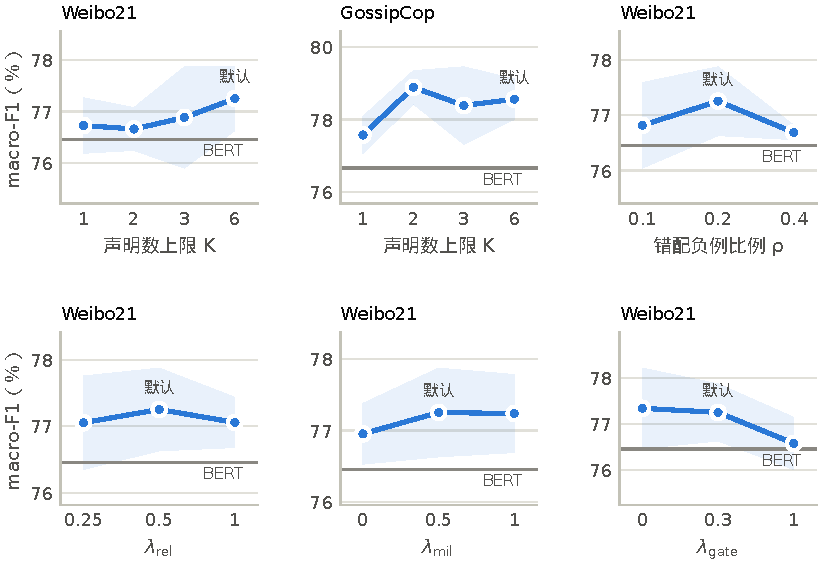
\includegraphics[width=\linewidth]{figures/sensitivity.pdf}
\caption{\method{} 对声明数上限 $K$（两个数据集）以及错配负例比例 $\rho$ 与三个损失权重（Weibo21）的敏感性。每个点为 3 个种子的均值，阴影为标准差；标“默认”的点是正文使用的取值在相同 3 个种子上的结果。灰色横线为 BERT。}\label{fig:sens}
\end{figure}

\section{受控测试集的构建细节}\label{app:perturb}

\paragraph{风格改写}
中文测试集 \cnt{CN/perturb/style_n} 条中有 \cnt{CN/perturb/style_rewritten} 条得到了可用的改写，英文 \cnt{EN/perturb/style_n} 条中为 \cnt{EN/perturb/style_rewritten} 条。被丢弃的主要是改写后长度超过原文 2.5 倍的短消息。作为事实保持程度的粗略代理，我们统计了原文中的数字串在改写后的保留比例：中文为 \pone{CN/fact_preservation/kept_rate}\%，英文为 \pone{EN/fact_preservation/kept_rate}\%。这只是一个代理指标，改写仍可能增删细节，这是 LLM 风格攻击的共同局限\citep{wu2024sheepdog}。

\paragraph{单句事实篡改}
候选为测试集中至少含两句、且存在长度足够的句子的真新闻（中文 \cnt{CN/perturb/tamper_candidates} 条，英文 \cnt{EN/perturb/tamper_candidates} 条）。篡改模型给出的片段必须在句中恰好出现一次，替换后字母与数字内容必须发生变化，且替换不得改变分句结果。最终得到中文 \cnt{CN/perturb/tamper_n} 条、英文 \cnt{EN/perturb/tamper_n} 条，平均每条分别含 \fone{CN/perturb/tamper_mean_sents} 与 \fone{EN/perturb/tamper_mean_sents} 句。按篡改类型的定位结果见表~\ref{tab:loc-type}。

\begin{table}[H]
\centering\small
\caption{按篡改类型划分的定位 Hit@1（\%）。}\label{tab:loc-type}
\fittable{tables/loc_type.tex}
\end{table}

\section{样例}\label{app:cases}

下面两条样例按预先固定的规则选出：篡改测试集中按编号排序、含 3--4 句且不超过 170 个字符的前两条，取随机种子 1 的模型输出，未做任何人工挑选。被篡改的句子与其原句用〔〕标出；表中 $+$ 与 $-$ 分别为 LLM 写出的支持论证与质疑论证。

\noindent\textbf{样例 1}（篡改类型：实体；\method{} 预测 $\hat y=0.00$）\par
{\small\begin{quote}
[1] \textbf{〔被篡改〕}【华为隐形指纹技术正式亮相】\quad\textbf{〔原句〕}【vivo隐形指纹技术正式亮相】\par
[2] 全面屏手机时代即将到来。\par
[3] 如此一来前后指纹已成为过去式，所有手机设计上又将站在同一起跑线了，大家觉得屏幕内指纹解锁帅不帅？秒拍视频\par
\end{quote}}
{\small\begin{tabularx}{\linewidth}{@{}clXccc@{}}
\toprule
句 & 类型 & 声明与两方论证 & $v_k$ & $g_k$ & $p_k$ \\
\midrule
-- & 整体 & \textbf{这条消息整体的可信度}\newline $+$ 全面屏手机的发展趋势确实存在。\newline $-$ 消息中提到的华为隐形指纹技术未得到官方证实。 & 0.74 & 0.23 & 0.00 \\
1 & 事实 & \textbf{华为隐形指纹技术正式亮相}\newline $+$ 华为经常发布新技术，此消息可能为谣言。\newline $-$ 华为官方未发布过此消息。 & 0.59 & 0.62 & 0.01 \\
2 & 观点 & \textbf{全面屏手机时代即将到来}\newline $+$ 手机厂商都在研发全面屏，此说法有一定合理性。\newline $-$ 全面屏技术仍在发展，尚未普及。 & 0.45 & 0.54 & 0.00 \\
\bottomrule
\end{tabularx}}
\par\medskip
\noindent\textbf{样例 2}（篡改类型：实体；\method{} 预测 $\hat y=0.00$）\par
{\small\begin{quote}
[1] 【天津健康码亮码超2100万次集成新功能后将沿用】\par
[2] 很多人关心疫情过后，天津健康码是否还会沿用？\par
[3] 在3月19日召开的新闻发布会上，天津市大数据管理中心主任边柯柯就此回应称，天津健康码将联合津心办一网通办平台，集成更多便民服务应用，继续沿用下去。\par
[4] \textbf{〔被篡改〕}边柯柯介绍说，天津将积极推动电子通行证在互联网+医疗健康相关场景的应用，实现签约预约\quad\textbf{〔原句〕}边柯柯介绍说，天津将积极推动健康码在互联网+医疗健康相关场景的应用，实现签约预约\par
\end{quote}}
{\small\begin{tabularx}{\linewidth}{@{}clXccc@{}}
\toprule
句 & 类型 & 声明与两方论证 & $v_k$ & $g_k$ & $p_k$ \\
\midrule
-- & 整体 & \textbf{这条消息整体的可信度}\newline $+$ 声明直接引用了官方发言，具有较高的可信度。\newline $-$ 消息中提及的具体日期和发言人姓名不明确，且部分内容为预测性意见，缺乏具体细节。 & 0.52 & 0.50 & 0.01 \\
3 & 引述 & \textbf{天津市大数据管理中心主任边柯柯在3月19日的新闻发布会上表示，天津健康码将集成更多便民服务应用，继续沿用下去。}\newline $+$ 该声明直接引用了官方发言，具有较高的可信度。\newline $-$ 新闻发布会的具体日期和发言人姓名未明确提及，可能存在信息不准确的风险。 & 0.23 & 0.82 & 0.01 \\
4 & 观点 & \textbf{天津将积极推动电子通行证在互联网+医疗健康相关场景的应用。}\newline $+$ 这是官方对未来发展的积极展望，符合政策导向。\newline $-$ 该说法是预测性意见，缺乏具体实施细节和时间表，可信度较低。 & 0.64 & 0.89 & 0.03 \\
\bottomrule
\end{tabularx}}
\par\medskip


\section{未使用的数据集}

LIAR-RAW 与 RAWFC 的价值在于为每条声明检索到的原始报道，闭卷条件下只剩一句很短的声明，且 \citet{thibault2025guide} 指出 LIAR 系列中有相当比例的样本本身不可核查；FakeNewsNet 的原始发布不含正文，只有标题与推文编号；SciFact 是需要证据文档的科学声明核查任务。它们与本文的闭卷、纯文本、新闻级检测设定不符，故未使用。


\end{document}
